\documentclass[master=elt,masteroption=eg,dutch,oneside]{kulemt}
\setup{title={DSP: Kleurconversie toepassen op een real time videosignaal},
  author={Gert-Jan Andries\and Xavier Dejager\and Nick Steen},
  promotor={Dries Debouvere},
  assessor={Dries Debouvere},
  assistant={Dries Debouvere}}

%\setup{font=lm}


\usepackage{graphicx}
\usepackage{titlesec}
\usepackage{listings}
\usepackage{color}
\usepackage{float}
\usepackage{amsmath}
\usepackage{booktabs}
\usepackage{upquote}
\usepackage{gensymb}
\usepackage{cite}
\usepackage{setspace}


\setlength{\parskip}{1em}
\setlength\parindent{0pt}

\titleformat{\chapter}[display]
    {\normalfont\huge\bfseries}{\chaptertitlename\ \thechapter}{20pt}{\Huge}
\titlespacing*{\chapter}{0pt}{-25pt}{10pt}


\definecolor{numberorange}{rgb}{1.0,0.4,0}
\definecolor{keywordblue}{rgb}{0.1,0.3,0.8}
\definecolor{commentgreen}{rgb}{0,0.5,0}
\definecolor{stringyellow}{rgb}{0.8,0.7,0}
\definecolor{mygray}{rgb}{0.4,0.4,0.4}

\lstset
{
  basicstyle=\ttfamily\footnotesize,
  commentstyle=\color{commentgreen},
  frame=single,
  numbers=left,
  numbersep=5pt,
  numberstyle=\tiny\color{mygray},
  keywordstyle=\color{keywordblue},
  showspaces=false,
  showstringspaces=false,
  stringstyle=\color{stringyellow},
  tabsize=2,
  breakatwhitespace=false,
  captionpos=b,
  keepspaces=true, 
  numbersep=2pt,
  showspaces=false, 
  showstringspaces=false,
  showtabs=false,
  tabsize=2,
  title=\lstname , 
  xleftmargin=2em,
  frame=single,
  framexleftmargin=1.5em,
  columns=flexible,
  breaklines=true
   %literate=%
   %{0}{{{\color{red}0}}}1
   %  {1}{{{\color{red}1}}}1
   %  {2}{{{\color{red}2}}}1
   % {3}{{{\color{red}3}}}1
   % {4}{{{\color{red}4}}}1
   % {5}{{{\color{red}5}}}1
   % {6}{{{\color{red}6}}}1
   % {7}{{{\color{red}7}}}1
   % {8}{{{\color{red}8}}}1
   % {9}{{{\color{red}9}}}1
}

%%%%%%%%%%%%%

\begin{document}


\tableofcontents*


%\listoffiguresandtables
\chapter{Afkortingen en symbolen}
\section*{Afkortingen}
\begin{flushleft}
  \renewcommand{\arraystretch}{1.1}
  \begin{tabularx}{\textwidth}{@{}p{12mm}X@{}}
    ALU & Arithmetic logic unit \\  
    AVF & Active video field \\ 
    cfr & Confer \\ 
    CPU & Central processor unit \\ 
    DAG & Data address generetor \\  
    DMA & Direct memory acces \\  
    DSP & Digital Signal Processing \\  
    EAV & End of active frame \\  
    Hz  & Hertz \\  
    IDE & Integrated development environment\\  
    ITU & International Telecommunication Union \\  
    kB  & Kilobyte \\ 
    MAC & Multiply and accumulate \\  
    MB  & Megabyte \\ 
    MHz & Megahertz\\ 
    NTSC & National Television System Committee \\  
    PAL &  Phase Alternating Line \\  
    PPI & Peripheral Parallel Interface \\  
    RGB & Rood Groen Blauw kleurenruimte \\
    RISC & Reduced instruction set computing \\ 
    SAV & Start of active frame\\ 
    SDRAM & Synchronous dynamic random access memory \\ 
    SIMD & Single instruction multiple data\\ 
    SRAM & Static random acces memory \\  
    TV   & Televisie \\ 
    YCbCr & zie YUV \\  
    YUV & Helderheid en Kleurvariatie kleurenruimte \\  
  \end{tabularx}
\end{flushleft}

 %\section*{Symbolen}
 %\begin{flushleft}
 %  \renewcommand{\arraystretch}{1.1}
 %  \begin{tabularx}{\textwidth}{@{}p{12mm}X@{}}
 %    pi   & 3.141592 \\
 %  \end{tabularx}
 %\end{flushleft}


% Nu begint de eigenlijke tekst
\mainmatter

\chapter{Inleiding}

\par DSP staat voor Digital Signal Processing, ofwel digitale signaalverwerking. Deze signalen kunnen zowel beeld- als audiomateriaal zijn, in dit labo is gekozen om het videodomein verder te bestuderen. De opdracht bestond uit de real-time verwerking en filtering van een videosignaal. Dit houdt onder meer in dat een signaal binnengelezen, geanalyseerd, gefilterd of aangepast en terug uitgestuurd moet worden, en dit in een zo kort mogelijke tijdspanne om de real-time factor te respecteren.

\par Gedurende het laboproject werd gewerkt met een beeldfragment van een aflevering van de Smurfen. In dit fragment dienen alle Smurfen een huidskleurverandering te ondergaan  zodat het uitgangssignaal een verzameling gele smurfen weergeeft. Het middel om dit te bereiken is de BlackFin EZ-Kit Lite met de BF-561 dual-core processor, met bijbehorende DSP++ IDE. Een krachtige processor in combinatie met een eenvoudige werkomgeving belooft een vlotte ervaring te geven.

\chapter{Doelstelling}

\par Het doel van dit DSP project is om met behulp van de Blackfin BF-561 DSP processor een kleurenconversie toe te passen op een realtime videosignaal. Dit videosignaal is afkomstig van een digitale camera en wordt via het NTSC protocol uitgestuurd. De kleursverandering die moet doorgevoerd worden is een transformatie van blauw (zoals bij de Smurfen) naar geel. 

\par Als voorbereiding voor dit labo werden reeds enkele DSP-algoritmes uitgevoerd in het simulatieprogramma Matlab. Aan de hand van de opgedane kennis kan het DSP alghoritme tijdens dit labo ge\"implementeerd worden op een DSP processor aan de hand van de programmeertaal C++.

\par Naast de praktische implementatie wordt er ook een studie gedaan naar kleurenruimtes en -converties, alsook een theoretische studie naar technieken die de performatie en de kwaliteit van het eindreslultaat kunnen vergroten door gebruik te maken van dezelfde hardware. Er werd dus theoretisch gezocht naar een zo performant mogelijk algoritme. 

	\begin{figure}[H]
		\centering
		
\includegraphics[width=0.85\textwidth]{Introduction/resultaat_smurf_2.png}
		\caption{Huidskleurverandering bij een smurf}
		\label{fig:smurf}
	\end{figure}



\chapter{BlackFin architectuur}
	
	\section{BlackFin processor algemeen overzicht}

		\par De BlackFin processorfamilie is een 16- of 32-bit microprocessor ontwikkeld door het bedrijf Analog Devices. De processor beschikt over een ingebouwde fixed-point DSP die wordt bijgestaan door twee 16-bit MACs. Hiernaast is er in de chip ook nog een kleine processor aanwezig. De BlackFin processorreeks is ook ontwikkeld met het oogpunt op low power functionaliteiten.

		\par De BlackFin gebruikt een 32-bit RISC microcontroller die ge\"implementeerd is op een SIMD architectuur. Een BlackFin core bevat twee 16-bit hardware MACs, twee 40-bit ALUs en een 40-bit barrel shifter. Deze opstelling zorgt ervoor dat er maximaal drie instructies per klokcyclus uitgevoerd kunnen worden. Om het aantal instructies te reduceren zijn er ook vier DAGs ingebouwd in de processor.

		\par De BlackFin maakt gebruik van een byte-adresseerbare flat memory map. Het level 1 en level 2 geheugen is ingebouwd in de processor en het level 3 geheugen dient extern toegevoegd te worden. Al deze geheugens zijn gemapt op 32-bit adressen. Dit zorgt er voor dat de BlackFin processoren opgebouwd zijn volgens de Von Neumann architectuur.

		\par Het level 1 intern SRAM geheugen, dat geklokt is op de snelheid van de processor, is gebaseerd op de Harvard architectuur. Het instructie- en datageheugen is verbonden met de processor via een gereserveerde databus. Het level 2 geheugen is trager geklokt dan de processor zelf. De codememory kan zowel in level 1 als in level 2 geheugen opgeslagen worden.

		\par De BlackFin processor beschikt over twee DMA-controllers die kunnen opereren tussen de peripherals en de verschillende geheugens binnen de processor. Dankzij deze DMA-controllers wordt de processor niet belast met het uitvoeren van data transfers in het geheugen.

	\section{BlackFin BF-561 processor}

		\par De BlackFin BF-561 die aanwezig is op het EZ-KIT Lite beschikt over twee processorkernen. De processor kan werken op een kloksnelheid van maximaal 600 Mhz. Verder beschikt deze processor over 328 kB intern geheugen (level 1 en level 2).  Hiernaast beschikt de processor over twee 12-kanaals DMA controllers om de geheugen-naar-geheugen operaties uit te voeren. In figuur~\ref{fig:bf561fbd} is een overzicht van de opbouw van de BlackFin BF-561 weergegeven. 

			\begin{figure}[H]
				\centering
				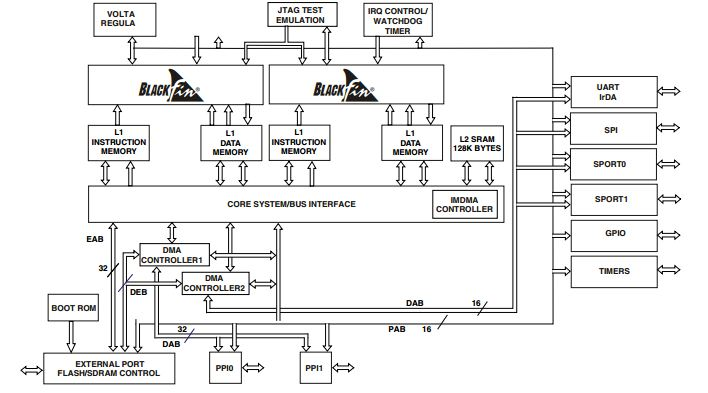
\includegraphics[width=0.95\textwidth]{Chapters/Chapter4/Images/bf-561.jpg}
				\caption{BF-561 functional block diagram}
				\label{fig:bf561fbd}
			\end{figure}

\chapter{Video Processing}

		%\par Er zijn verschillende mogelijkheden om video- en imageprocessing toe te passen met behulp van de BlackFin processoren. In de vlgende hoofdstukken worden drie van deze technieken kort omschreven. 
		
	\section{Interframe processing}
		
		\par Interframe processing wordt toegepast wanneer er een afhankelijk verband is tussen de verschillende frames. Dit is bijvoorbeeld het geval wanneer een inkomend frame vergeleken moet worden met een referentie frame. Het level 1 en 2 geheugen van de BlackFin processor zijn onvoldoende groot om deze frames in op te slaan. Er dient dus gebruik gemaakt te worden van het level 3 SDRAM. Het nadeel aan dit SDRAM geheugen is dat het veel trager is dan het ingebouwde level 1 en 2 geheugen van de processor zelf.  Een frame wordt onderverdeeld in verschillende delen die een sub block genoemd worden. Deze sub blocks worden vervolgens getransfereerd naar het level 1 geheugen van de BlackFinprocessor om verwerkt te worden. Indien het level 1 geheugen nog te klein blijkt te zijn kan het level 2 geheugen gebruikt worden als tussenbuffer. Alle geheugenoperaties worden uitgevoerd door de DMA-controller. In figuur~\ref{fig:interframe_processing} wordt een voorbeeld weergegeven van de hierboven beschreven techniek. Er bestaat een afhankelijkheid tussen currentframe en referenceframe.

			\begin{figure}[H]
				\centering
				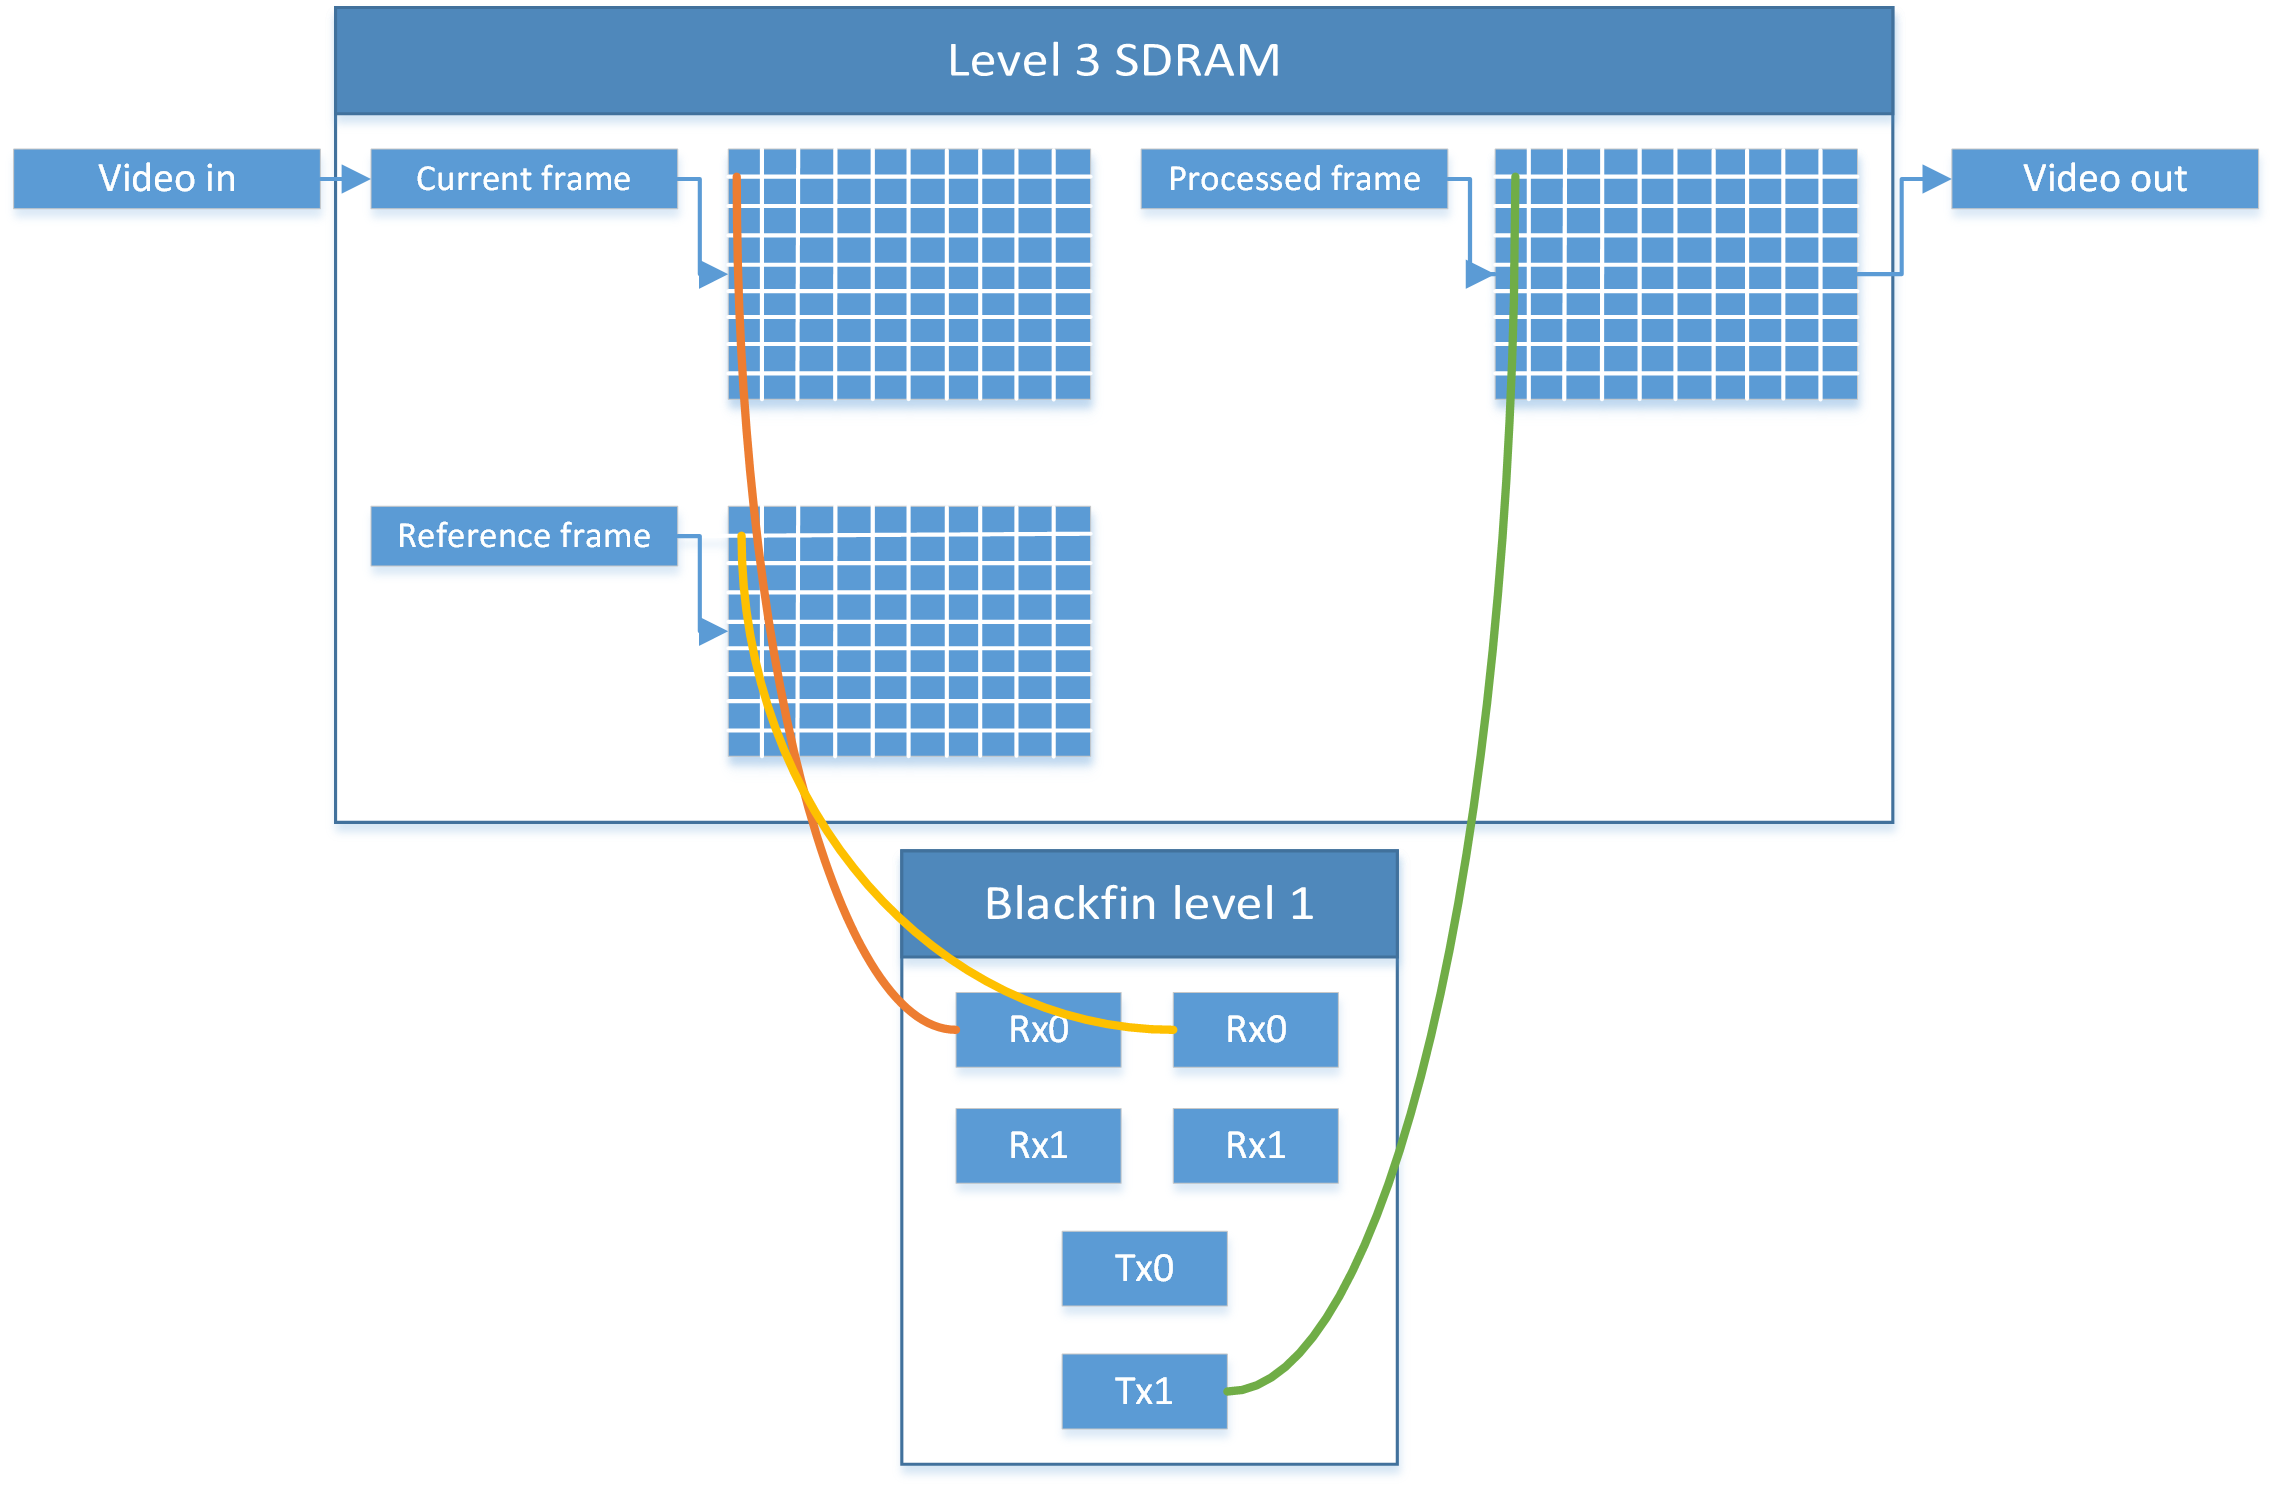
\includegraphics[width=0.90\textwidth]{Chapters/Chapter4/Images/DMA_interframe_processing.png}
				\caption{Interframe processing data flow diagram}
				\label{fig:interframe_processing}
			\end{figure}

	\section{Line processing}

		\par Bij het line processing principe wordt frame per frame te werk gegaan. Het frame zal in een eerste stap opgehaald worden uit het geheugen van de peripheral. Nadat een frame opgehaald is wordt het lijn per lijn verplaatst naar het level 1 geheugen van de BlackFin. Deze actie gebeurt door middel van de DMA-controller zodat de processor hier geen hinder van ondervindt.

		\par Een nog effici\"entere methode is om de data onmiddelijk van de peripheral lijn per lijn naar het level 1 geheugen te transfereren. Na der verwerking moet ook de data terug verstuurd worden naar een peripheral om deze weer te geven. Dit kan ook onmiddelijk lijn per lijn vanuit het level 1 geheugen, maar ook via het level 3 geheugen waar een volledig frame gebufferd kan worden. 

		\par In figuur~\ref{fig:line_processing} wordt de opbouw van een lijn-gebaseerde aanpak weergegeven. De DMA wordt gebruikt om data onmiddelijk naar het level 1 geheugen van de BlackFin te transfereren. Vervolgens wordt door de BlackFin een actie uigevoerd op de videolijn die dan weer wordt getransfereerd van het level 1 geheugen naar de video encoder. Deze transfers gebeuren door middel van de DMA-controlller. De dubbele buffering in het level 1 geheugen zorgt ervoor dat de DMA en de processing door de BlackFin processor concurrent uitgevoerd kunnen worden. Op deze manier kan video in realtime verwerkt worden.

			\begin{figure}[H]
				\centering
				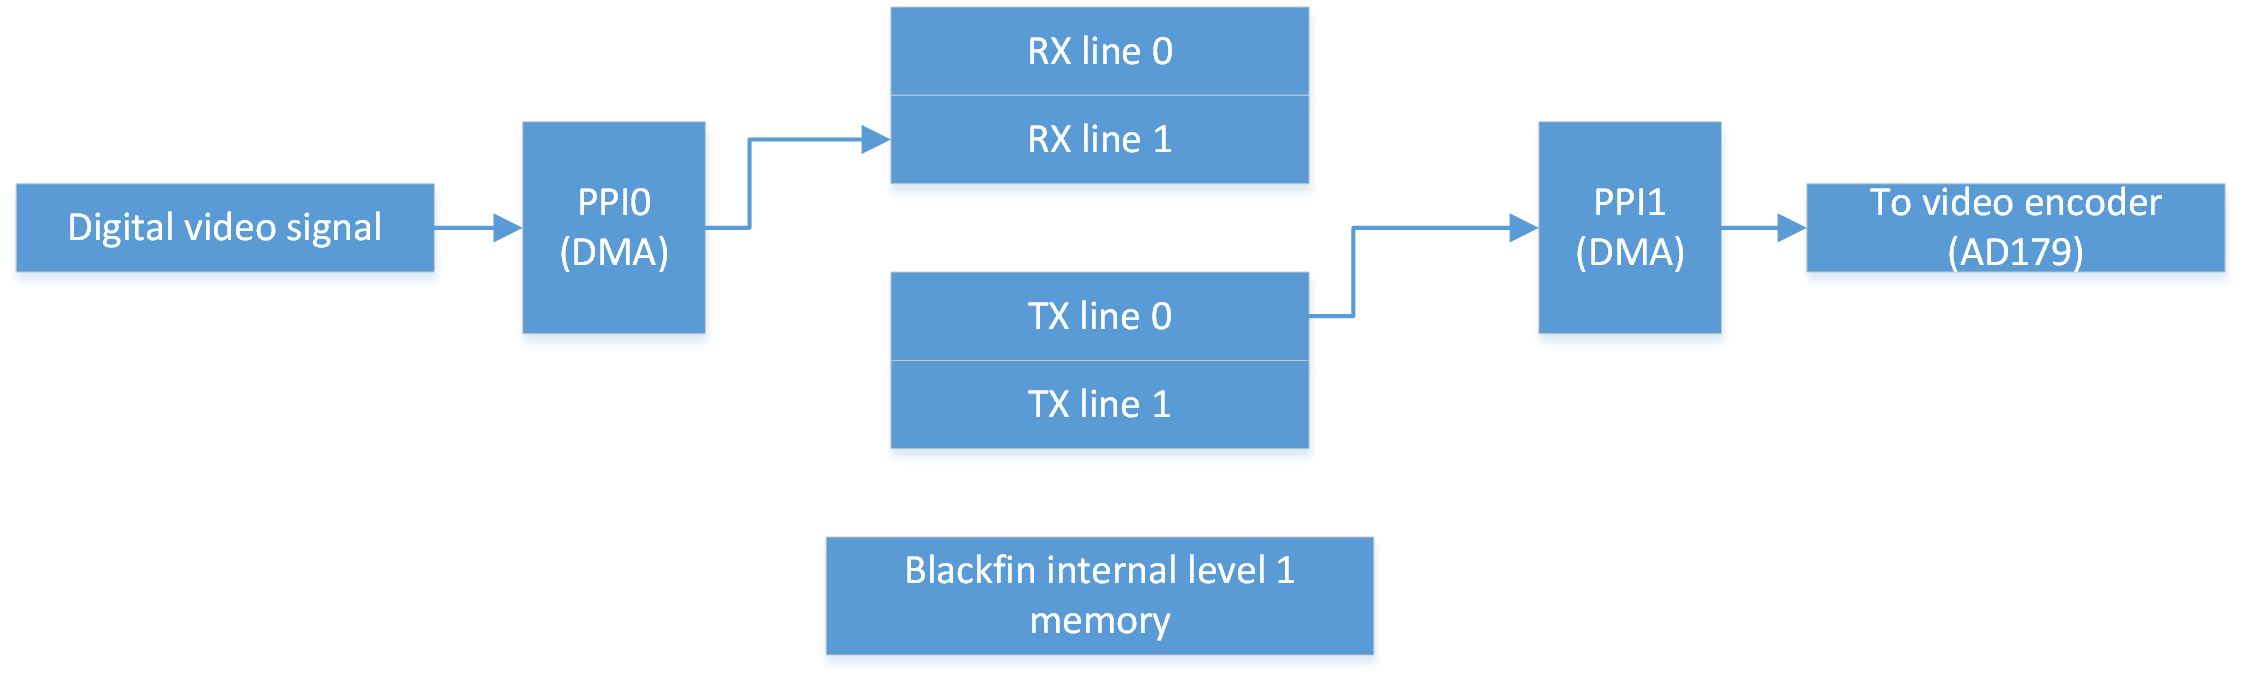
\includegraphics[width=0.95\textwidth]{Chapters/Chapter4/Images/DMA_line_processing.png}
				\caption{Line processing data flow diagram}
				\label{fig:line_processing}
			\end{figure}
	\newpage
	\section{Macro block processing}
		
		\par Bij macro block processing wordt het frame niet in zijn geheel verwerkt, maar opgedeeld in verschillende secties. Elke sectie heeft een dimensie van n bij m. De hoogte van de macroblock wordt weergegeven door n en de breedte door m. Het level 1 geheugen van de BlackFinprocessor is te klein om een alle n-lijnen van een afbeelding op te slaan, daarom wordt gebruik gemaakt van het level 2 geheugen. Dit zorgt ervoor dat er minder bandbreedte van de databus gebruikt wordt. 

		\par Ook bij het level 2 gheugen is de opslagcapaciteit beperkt. Een volledige afbeelding past vaak niet in het level 2 geheugen. Daarom wordt slechts een aantal lijnen van de afbeelding (n lijnen) in het level 2 geheugen geplaatst. Dit gebeurt door middel van de parallel peripheral interface van de DMA. Vervolgens zullen macroblocks verplaatst worden van het level 2 geheugen naar het level 1 geheugen waar deze verwerkt kunnen worden door de BlackFin processor. Er vindt een dubbele buffering plaats in zowel het level 1 als het level 2 geheugen. Telkens wordt de DMA-controller gebruikt voor deze geheugenoverdracht zodat de processor hier geen hinder van ondervindt.

		\par In figuur~\ref{fig:block_processing} is een voorbeeldopstelling te zien van macro block processing. In dit voorbeeld worden twee DMA-controllers gebruikt om de dataoverdrachten uit te voeren. Er wordt ook een dubbele framebuffering voorzien om de processwindow te vergroten.

			\begin{figure}[H]
				\centering
				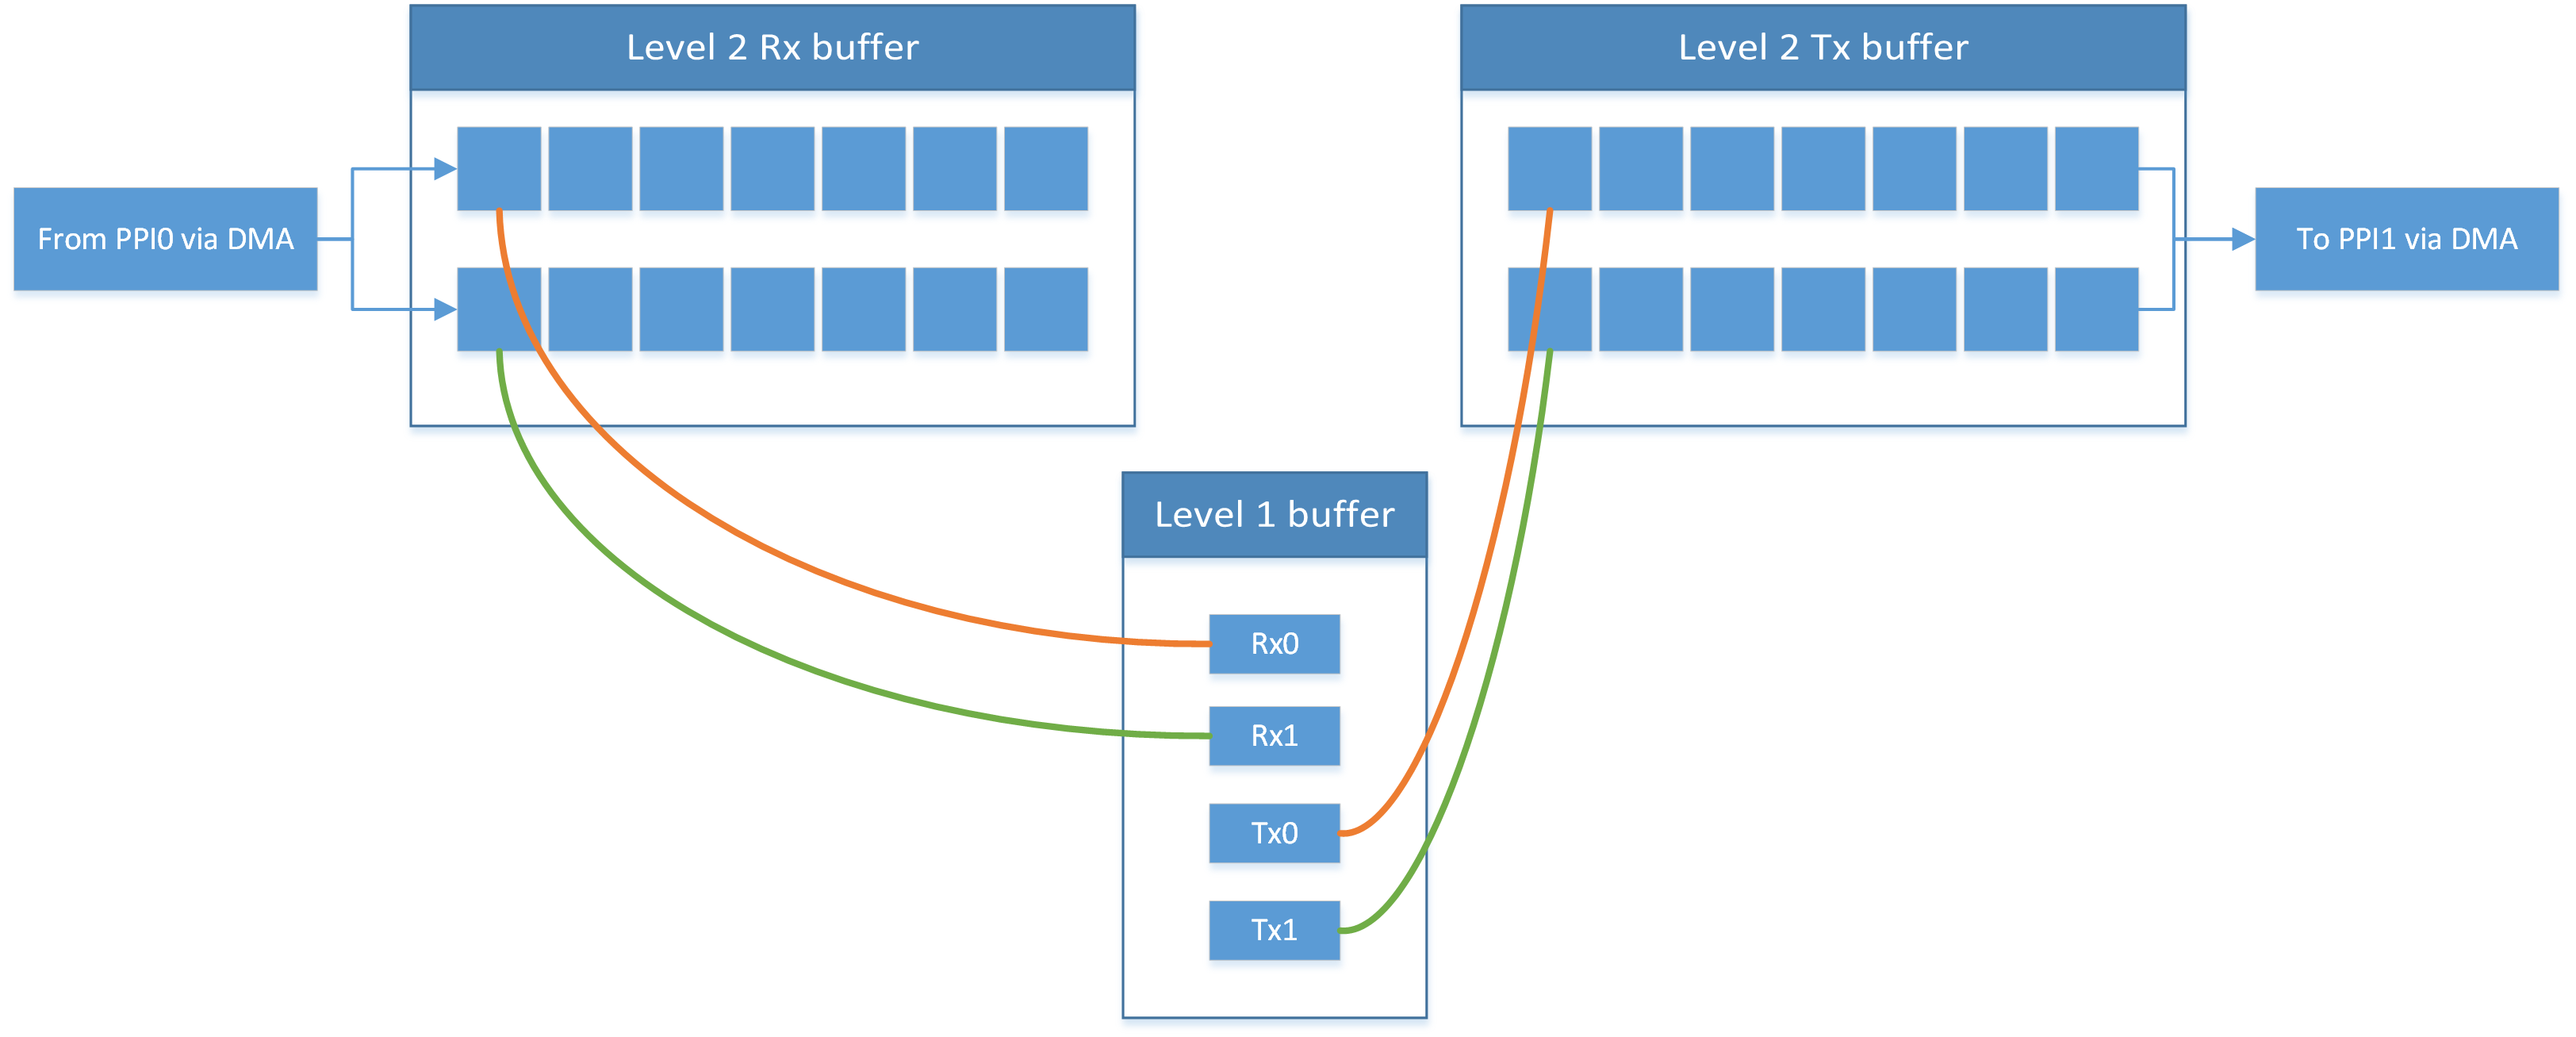
\includegraphics[width=0.95\textwidth]{Chapters/Chapter4/Images/DMA_block_matrix.png}
				\caption{Macro block processing data flow diagram}
				\label{fig:block_processing}
			\end{figure}
	\newpage
	\section{Optimalisatie}
		
		\par Door bij het design rekening te houden met de architectuur van de BlackFin processor kan er flink wat snelheid gewonnen worden. In de paragrafen hieronder worden enkele design tips kort toegelicht.

		\par Wanneer men via een DMA-controller data wil verplaatsen van het ene geheugen naar het andere geheugen dient men rekening de houden met de breedte van de data bus. Bij de BlackFin BF-56x reeks is er een 32-bit brede databus voorzien. Door de DMA-controller zo in te stellen dat hij per operatie telkens 32-bit of een veelvoud daarvan moet verplaatsen, wordt er optimaal gebruik gemaakt van de DMA en databus.

		\par Om de DMA-controllers effici\"ent te gebruiken dient men er rekening mee te houden bij het ontwerp dat nooit twee geheugentransferts plaatsvinden op het zelfde moment binnen eenzelfde DMA kanaal. 

		Bronnen:~\cite{bib_6},~\cite{bib_8},~\cite{bib_10},~\cite{bib_11}.



\chapter{Video Input}

\section{Beeldformaat}
	\subsection{Video frame}
		\par De video input is een stream van frames die elk een beeld voorstellen. De NTSC standaard, gedefinieerd volgens ITU-R BT656~\cite{bib_3}~\cite{bib_4}, legt een framerate van 60Hz op, dus 60 frames per seconde. Elk frame bestaat uit verschillende lijnen data, zichtbare en onzichtbare. De zichtbare lijnen zijn gegroepeerd per even en oneven regels, en zijn dus in twee velden, Active Video Fields (AVF), terug te vinden in het binnekomende frame. De overige, en dus onzichtbare lijnen, zorgen voor synchronisatie tussen de bron en de weergever. Deze regels worden ook blanking lines genoemd. Hoe de lijnen precies voorkomen in een frame is te vinden in figuur~\ref{fig:OpbouwFrameImage}.
		
		\begin{figure}[H]
			\centering
			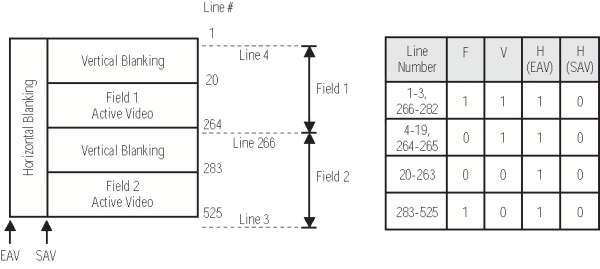
\includegraphics[width=0.95\textwidth]{Chapters/Chapter1/Images/Frame.png}
			\caption{Opbouw ITU-R BT656 frame~\cite{bib_15}}
			\label{fig:OpbouwFrameImage}
		\end{figure}

		\par Er is duidelijk te zien dat er eerst een groep lijnen komt die de vertical blanking lijnen voorstellen. Deze regels gaven de vroegere CRT televisietoestellen de tijd om hun beam van beneden tot weer volledig boven te bewegen. Aangezien de nieuwere toestellen niet meer met een kathodestraalbuis werken, maar over een volledig digitaal verwerkingssysteem beschikken, kan deze data overschreven worden met timingintervallen of andere metadata. Er kan dus data meegestuurd worden binnenin de blanking intervallen, maar deze wordt door vele toestellen uitgefilterd om interferentie van beeldlijnen te voorkomen.

		\par De vertical blanking is opgevolgd door het eerste AVF. Deze eerste groep bevat de oneven lijnen van het zichtbare beeld.
		Hoe een lijn precies in elkaar zit wordt in het volgende onderdeel verder beschreven, hier beperken we ons tot de adressering van de lijnen binnen het frame. Dit eerste AVF is gevolgd door opnieuw een vertical blanking en een AVF. Een ITU-R BT656 frame bestaat uit 525 opeenvolgende lijnen. Aangezien het zictbare beeld 480 lijnen telt, blijven er 48 lijnen over die kunnen dienen voor vertical blanking, wat duidelijk overeenkomt met figuur~\ref{fig:OpbouwFrameImage} op pagina ~\pageref{fig:OpbouwFrameImage}.

	\subsection{Structuur van een beeldlijn}
	\label{subsec:LijnSubSec}
		\par Er zijn twee soorten lijnen, de zichtbare en de onzichtbare. Ze delen eenzelfde opbouw, maar hebben een groot verschil, namelijk dat de zichbare lijnen een AVF bevatten waar de onzichtbare lijnen een vertical blanking field bevatten. Zowel de headers als de lijnlengte zijn exact gelijk en kunnen dus beschouwd worden als eenzelfde opeenvolging van data. Men moet er bij het verwerken wel voor zorgen dat er niet over de vertical blanking geschreven wordt op willekeurige plaatsen, omdat dit ongewenste effecten kan hebben, afhankelijk van het type toestel waarop het beeld weergegeven wordt.

		\begin{figure}[H]
			\centering
			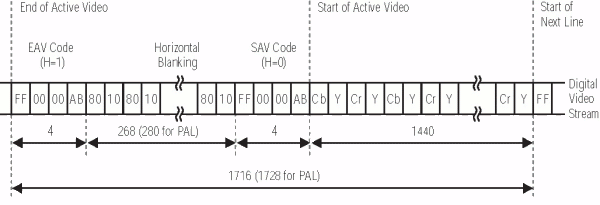
\includegraphics[width=0.95\textwidth]{Chapters/Chapter1/Images/Line.png}
			\caption{Opbouw ITU-R BT656 lijn ~\cite{bib_16}}
			\label{fig:OpbouwLijnImage}
		\end{figure}

		\par Een lijn bestaat uit verscheidene elementen: EAV code, horizontal blanking, SAV code en data. De EAV code heeft een lengte van 4 bytes en bestaat uit drie bytes met een vaste waarde (0xFF 0x00 0x00), gevolgd door een vierde byte die aanduidt of de data die volgt bestaat uit de even of oneven lijnen, alsook de status van de blanking. Op deze manier weet het toestel of de lijn een blanking, al dan niet een beeldlijn voorstelt. De blanking die erop volgt is opgebouwd uit een continue opvolging van 0x80 0x10, en dit voor een lengte van 268 bytes. Deze data zorgt voor de horizontale uitlijning van het beeld. De SAV code staat voor Start of Active Video en dient dus om aan te tonen dat de een AVF zal starten zodra de SAV code voorbij is. Deze heeft opnieuw een lengte van 4 bytes, bestaande uit drie vaste bytes (0xFF 0x00 0x00) gevolgd door een code die aanduidt welke data er zal volgen, zijnde welk field (even of oneven) en de blanking status.
		Als laatste is er dus de effectieve lijndata, met een lengte van 1440 bytes. Deze 1440 bytes stellen een volledige lijn voor, zij het even of oneven, en tellen dus 720 pixels, wat neerkomt op 2 bytes per pixel. Er is een opvolging van Cb Y Cr Y over de volledige lengte, hoe dit formaat precies gestructureerd is wordt in het volgende hoofdstuk besproken.

\section{Kleurenruimte}
	\subsection{RGB}
		\par RGB is de meest gekende en voor de hand liggende kleurenruimte, ze bestaat uit een combinatie van de 3 kleuren Rood, Groen en Blauw en is voor de gebruiker ook de meest eenvoudige manier om een kleur te omschrijven. Er bestaan echter verschillende formaten van deze RGB standaard, vaak gekozen om datacompressie toe te passen waar mogelijk. Als we RGB als een 24 bits getal zien van telkens 8 bits per kleurwaarde, kunnen we heel eenvoudig een kleur detecteren en deze aanpassen. Cfr.~\ref{subsec:KleurConversieSubSec} voor de omzetting van RGB naar YCbCr en omgekeerd. Op figuur~\ref{fig:RGBColorSpaceImage} is te zien hoe deze kleurruimte kan worden voorgesteld.

		\par Een kleur aanpassen in deze ruimte is vrij voor de hand liggend, aangezien het een voorstelling is die we gewoon zijn. We kunnen de componenten namelijk perfect apart waarnemen en ons voorstellen. Op die manier kunnen we dan ook meteen voor ons zien wat er zal gebeuren als een aanpassing zouden doen aan \'e\'en van de componenten.

		\begin{figure}[H]
			\centering
			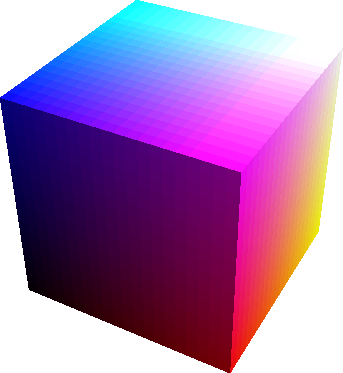
\includegraphics[width=0.35\textwidth]{Chapters/Chapter1/Images/RGBspace.png}
			\caption{RGB kleurenruimte~\cite{bib_17}}
			\label{fig:RGBColorSpaceImage}
		\end{figure}
		
		\par Stel dat we een RGB kleur (97,179,254) hebben, en we willen hierop een transformatie uitvoeren dan hebben we reeds alle kleuren ter beschikking. Indien we de helderheid willen opdrijven moeten we alle drie de waarden aanpassen, namelijk verhogen met eenzelfde factor. Het tegenovergestelde geldt voor het verdonkeren van de kleur.
		\par Willen we een kleurverandering doorvoeren, zoals dit met deze opdracht het geval is met blauw en geel, blijft dit toch nog een vrij complexe operatie. In het geval we blauw willen converteren naar geel moeten we de rode en de groene component vergroten terwijl we de blauwe component drastisch laten inkrimpen. In pseudocode kan dit verwezenlijkt worden op de volgende manier:
		\bigskip
   		\begin{lstlisting}[language=VBScript, caption=Pseudocode voor het vervangen van blauw met geel]
if 0>R>115 and 100>G>200 and 0>B>255
   	R = 255
   	G = 255
   	B = 0
end		\end{lstlisting}

		Dit levert echter een monotoon geel op, wat voor de ogen niet zo aangenaam is om naar te kijken. Daarom kiezen we om de (R,G,B) componenten geen exacte nieuwe waarde te geven, maar \'e\'en die afhankelijk is van hun oorspronkelijke waarde. Dit kunnen we doen door de waarden met een vaste maat te vergroten of verkleinen, vertrekken van de waarde die de pixel reeds heeft.
		\bigskip
		\begin{lstlisting}[language=VBScript, caption=Pseudocode voor het vervangen van blauw met geel met behoud van tinten]
if 0>R>115 and 100>G>200 and 0>B>255
	R = 255
	G = min(G+54, 255)
	B = max(B-215,0)
end		\end{lstlisting}

	\newpage
	\subsection{YCbCr}
	\label{subsec:YCbCrSubSec}
		\par YCbCr is geen echte kleurenruimte, maar een formaat om een kleurenruimte te transporteren van een bron naar een scherm, het is gebruikt in het ITU-R BT656 formaat en is ontworpen om een zelfde kleurervaring te leveren in slechts 16 bits per pixel in plaats van 24 bij standaard RGB. Eigenlijk is het niet volledig correct om van 16 bits per pixel te spreken, aangezien we eigenlijk 32 bits per 2 pixels gebruiken~\cite{bib_2}. Twee naast elkaar liggende pixels delen eenzelfde Cb en Cr waarde, terwijl ze elk een eigen Y-waarde bevatten. Het menselijk oog is namelijk veel gevoeliger voor veranderingen in helderheid dan voor veranderingen in kleur. Op figuur~\ref{fig:YCbCrColorSpaceImage} is te zien hoe deze kleurruimte kan worden voorgesteld.

		\begin{figure}[H]
			\centering
			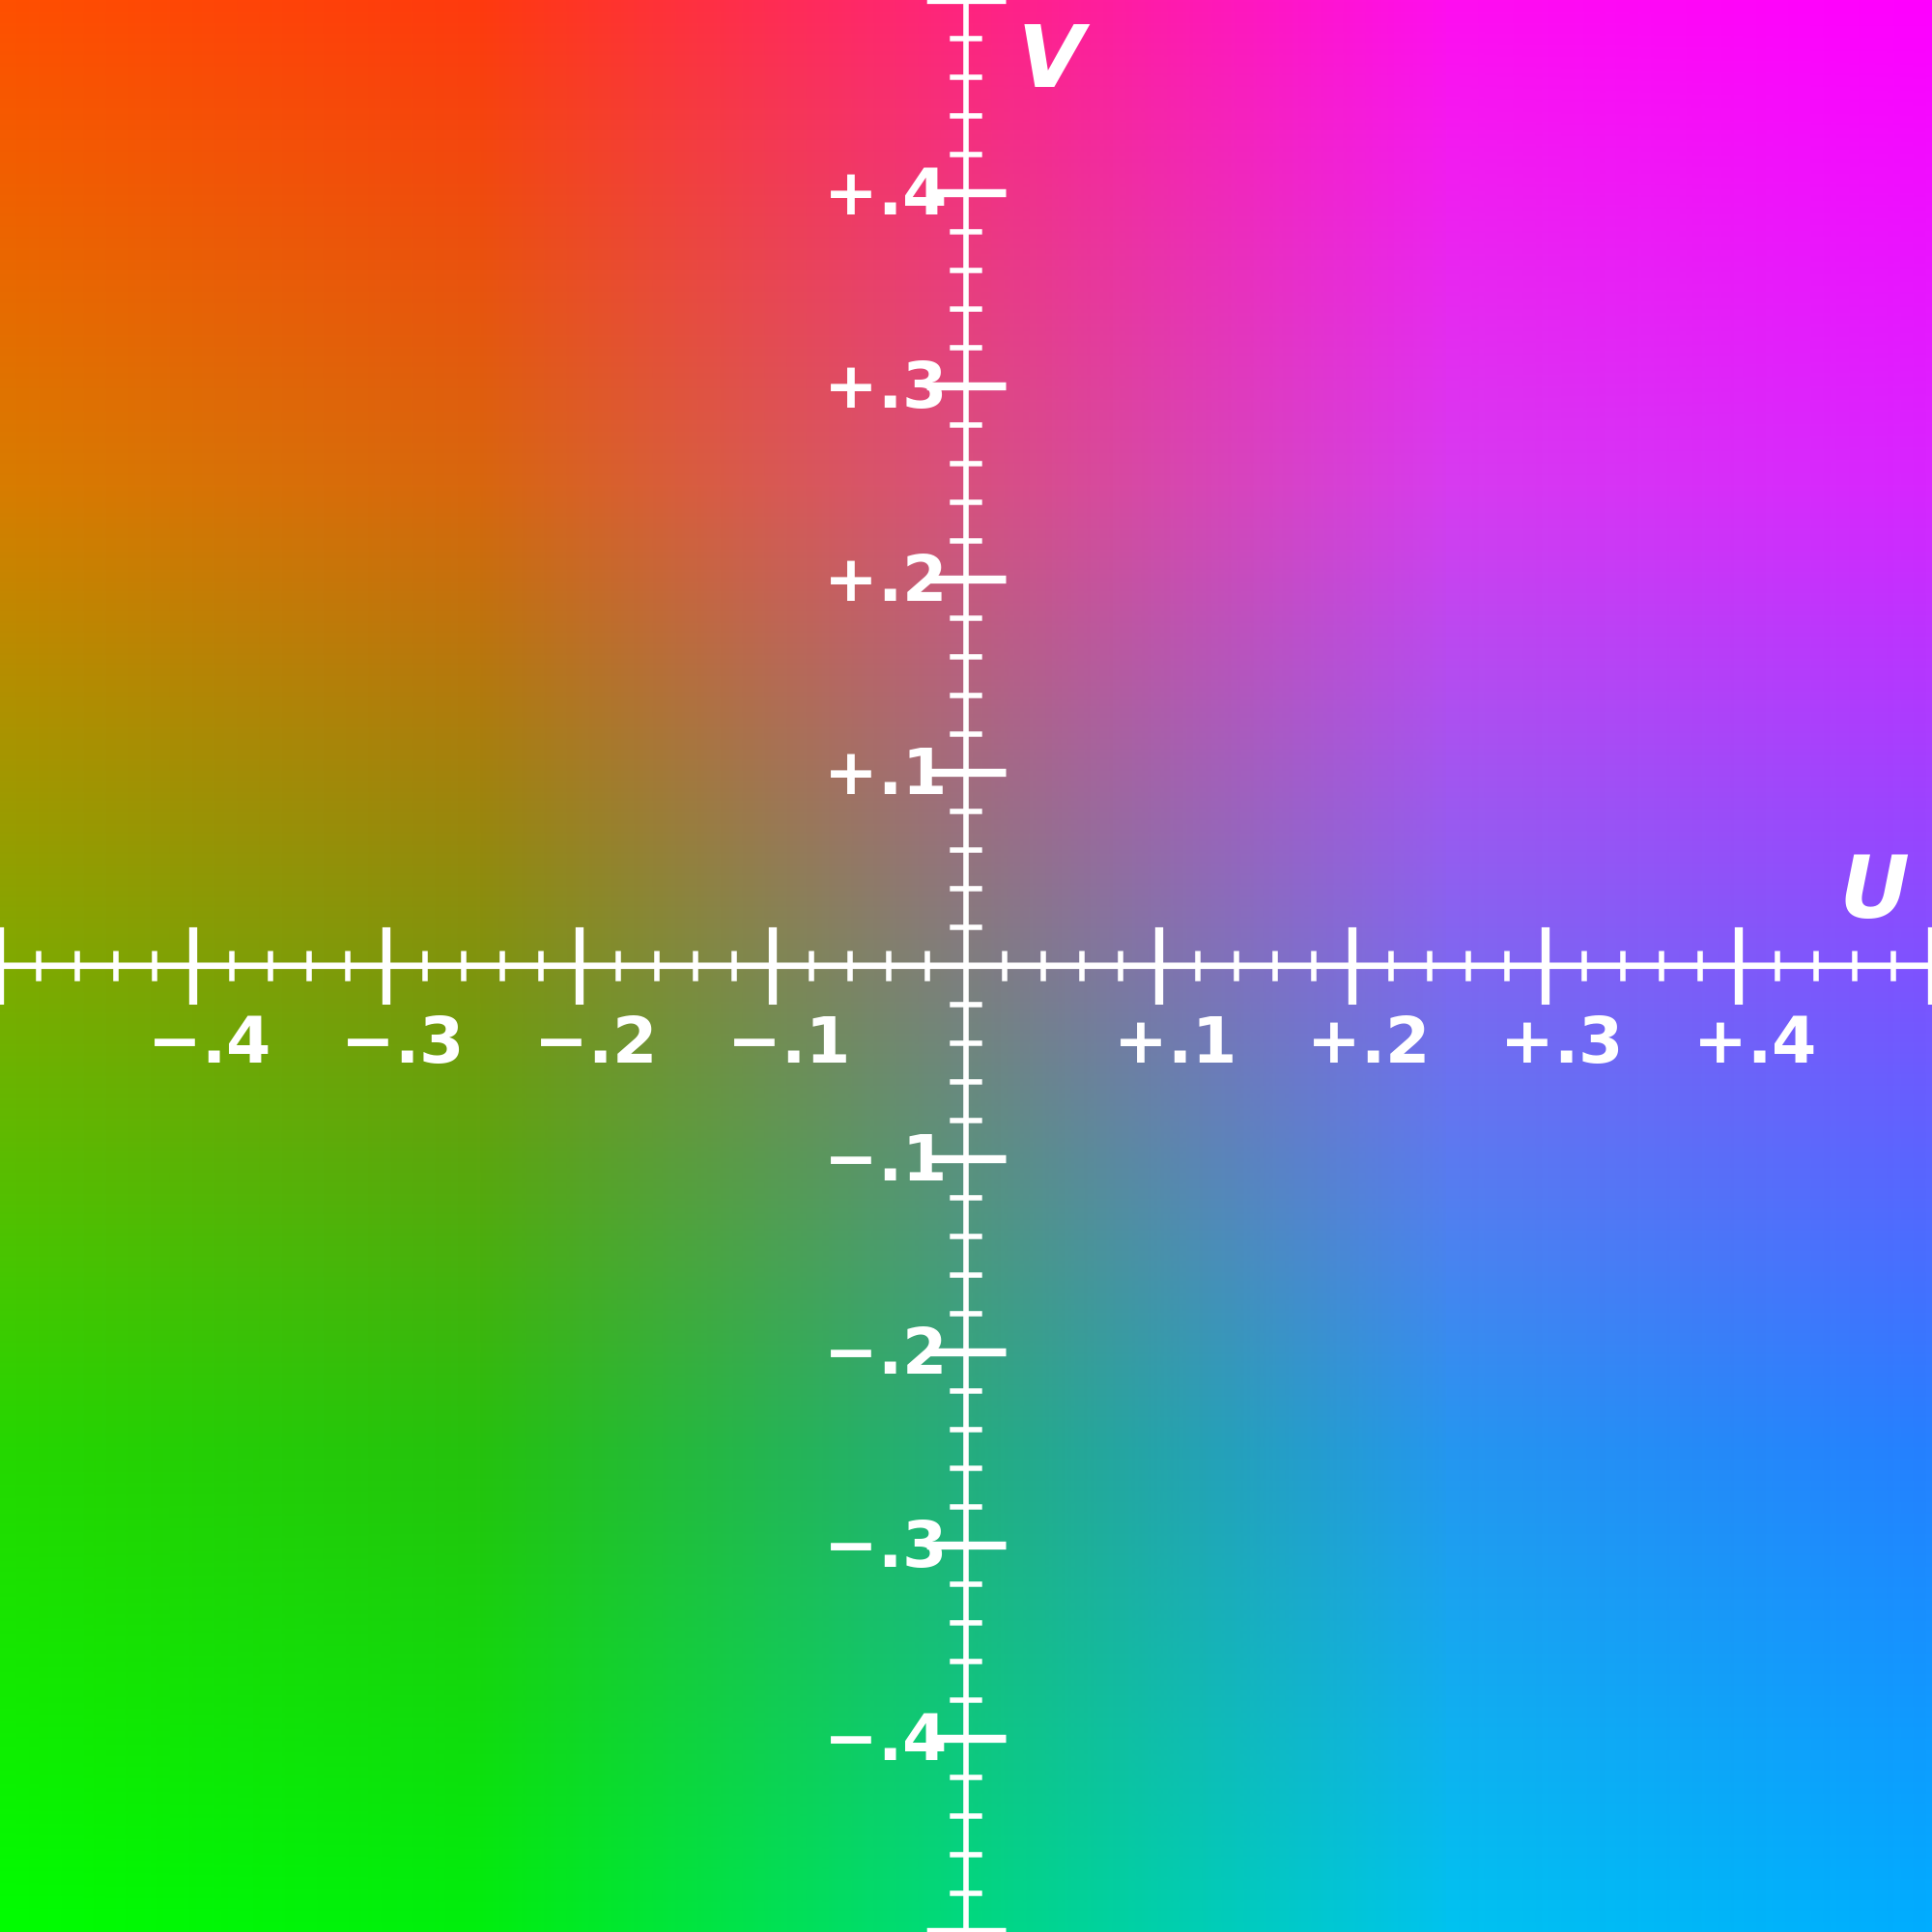
\includegraphics[width=0.4\textwidth]{Chapters/Chapter1/Images/YUVspace.png}
			\caption{YCbCr Kleurenruimte~\cite{bib_18}}
			\label{fig:YCbCrColorSpaceImage}
		\end{figure}

		\par Het vervangen van een kleur in het YCbCr formaat is heel wat complexer omdat het kleurenbereik dat we nodig hebben om een Smurf volledig naar geel te wijzigen, zo groot is dat we andere kleuren ook mee converteren. Grijstinten zijn een voorbeeld van deze bijkomende kleuren. Het afstellen van het bereik is dus veel preciezer, maar door te precies te werk te gaan verliezen we een deel van het blauwe spectrum waardoor de kans bestaat dat niet alle blauw gezien wordt als binnen de grenzen liggend. Het algoritme ziet er in pseudocode als volgt uit:
		\bigskip
		\begin{lstlisting}[language=VBScript, caption=Pseudocode voor het vervangen van blauw door geel]
if Y >= 130 and Y <= 180 and Cb > 150 and Cr > 50 and Cr < 100)
	Y = 0xEB
	Cb = 0x28
	Cr = 0x98
end		\end{lstlisting}

	\subsection{Conversie}
	\label{subsec:KleurConversieSubSec}
		\par Voor de conversie van RGB naar YCbCr en omgekeerd zijn er enkele vaste formules die gehanteerd kunnen worden. Aan de hand van de samenstelling van een lijn kunnen we dus uit 4 bytes data van het Active Video Frame 2 pixels halen. Deze waarden kunnen dan via de volgende formules~\cite{bib_1} geconverteerd worden tussen beide formaten:
   		
   		\begin{table}[H]
			\centering
				\begin{tabular}{@{}l|l@{}}
					\toprule
					RGB to YCbCr&YCbCr to RGB  \\ \midrule
					$R = Y + 1.140V$&$Y =  0.299R + 0.587G + 0.114B$ \\
					$G = Y - 0.395U - 0.581V$&$U = -0.147R - 0.289G + 0.436B$  \\
					$B = Y + 2.032U$&$V =  0.615R - 0.515G - 0.100B$ \\ \bottomrule
				\end{tabular}
			\caption{Formules RGB en YCbCr conversie ~\cite{bib_1}}
			\label{tab:RGBYCbCrFormulesTable}
		\end{table}

		\par Kleurenconversie tussen deze twee ruimtes is dus prefect mogelijk in beide richtingen. In ideale omstandigheden kunnen we dus voor deze opdracht de YCbCr waardes binnenlezen voor twee naast elkaar liggende pixels, en deze converteren naar twee RGB pixels. We laten het algoritme om de blauwe kleur te veranderen in geel inwerken op beide van deze pixels, en converteren deze opnieuw naar de YCbCr ruimte om ze dan terug in het frame te plaatsen en weer uit te sturen.
		\bigskip
		\begin{lstlisting}[language=VBScript,caption=Pseudocode voor een kleurconversie en -vervanging van blauw naar geel]
R = Y + 1.140V
G = Y - 0.395U - 0.581V
B = Y + 2.032U

if 0>R>115 and 100>G>200 and 0>B>255
	R = 255
	G = min(G+54, 255)
	B = max(B-215,0)
end

Y =  0.299R + 0.587G + 0.114B
U = -0.147R - 0.289G + 0.436B
V =  0.615R - 0.515G - 0.100B		\end{lstlisting}

		\par Na wat experimenteren zijn we echter tot de conclusie gekoment dat deze ideale omstandigheden niet bestaan, of toch niet in deze situatie. De processor is namelijk niet in staat om binnen de tijd van \'e\'en enkel frame over alle pixels te itereren en deze conversie uit te voeren. Aangezien het omzetten gebruikt maakt van floating point operaties neemt dit te veel tijd in beslag om op tijd klaar te zijn. Het zal dus noodzakelijk zijn om de kleurwijziging uit te voeren binnen de YCbCr kleurenruimte. Dit brengt echter heel wat nadelen met zich mee, cfr.~\ref{subsec:YCbCrSubSec} op pagina~\pageref{subsec:YCbCrSubSec}.

\section{Kleurbepaling van een Smurf}

	\par De kleur van een Smurf werd aan de hand van het programma Photoshop bepaald in de RGB kleurenruimte. Een Smurf heeft geen solide kleur dus werd er een bereik bepaald waarbinnen een kleur moet vallen om als Smurfenblauw gedetecteerd te worden. Deze RGB kleurwaarden werden door middel van het programma Matlab geconverteerd naar de YCbCr kleurenruimte volgens de formules die eerder in dit hoofdstuk besproken werden. De grenzen worden weergegeven in tabel~\ref{tbl:huidskleurwaarden}.

		\begin{table}[h]
			\centering
			\begin{tabular}{l|cc}
			\multicolumn{1}{c}{} & Minimum waarde & Maximum waarde \\
			\hline
			Y                    & 130            & 180            \\
			Cb                   & 150            & 240            \\
			Cr                   & 50             & 100            \\
			\hline
			\hline
			R                    & 8              & 146            \\
			G                    & 187            & 170            \\
			B                    & 177            & 255        	   \\
			\hline   
			\end{tabular}
		\caption{Bereik van de huidskleurwaarden van een Smurf}
		\label{tbl:huidskleurwaarden}
		\end{table}


\newpage
\chapter{Implementatie}

\par In de volgende hoofdstukken wordt besproken hoe het eindresultaat bereikt werd. De werkwijze is stapsgewijs en in elke stap wordt er verder geoptimaliseerd. In de eerste stappen was er nog sprake van een kleurenconversie van YCbCr naar RGB, maar deze werd later weggelaten om aan snelheid te winnen. In het definitieve ontwerp wordt dus volledig gewerkt in de YCbCr kleurenruimte met het oog op de snelheid van de frameprocessing.

\section{Algemeen overzicht}

	\begin{figure}[H]
			\centering
			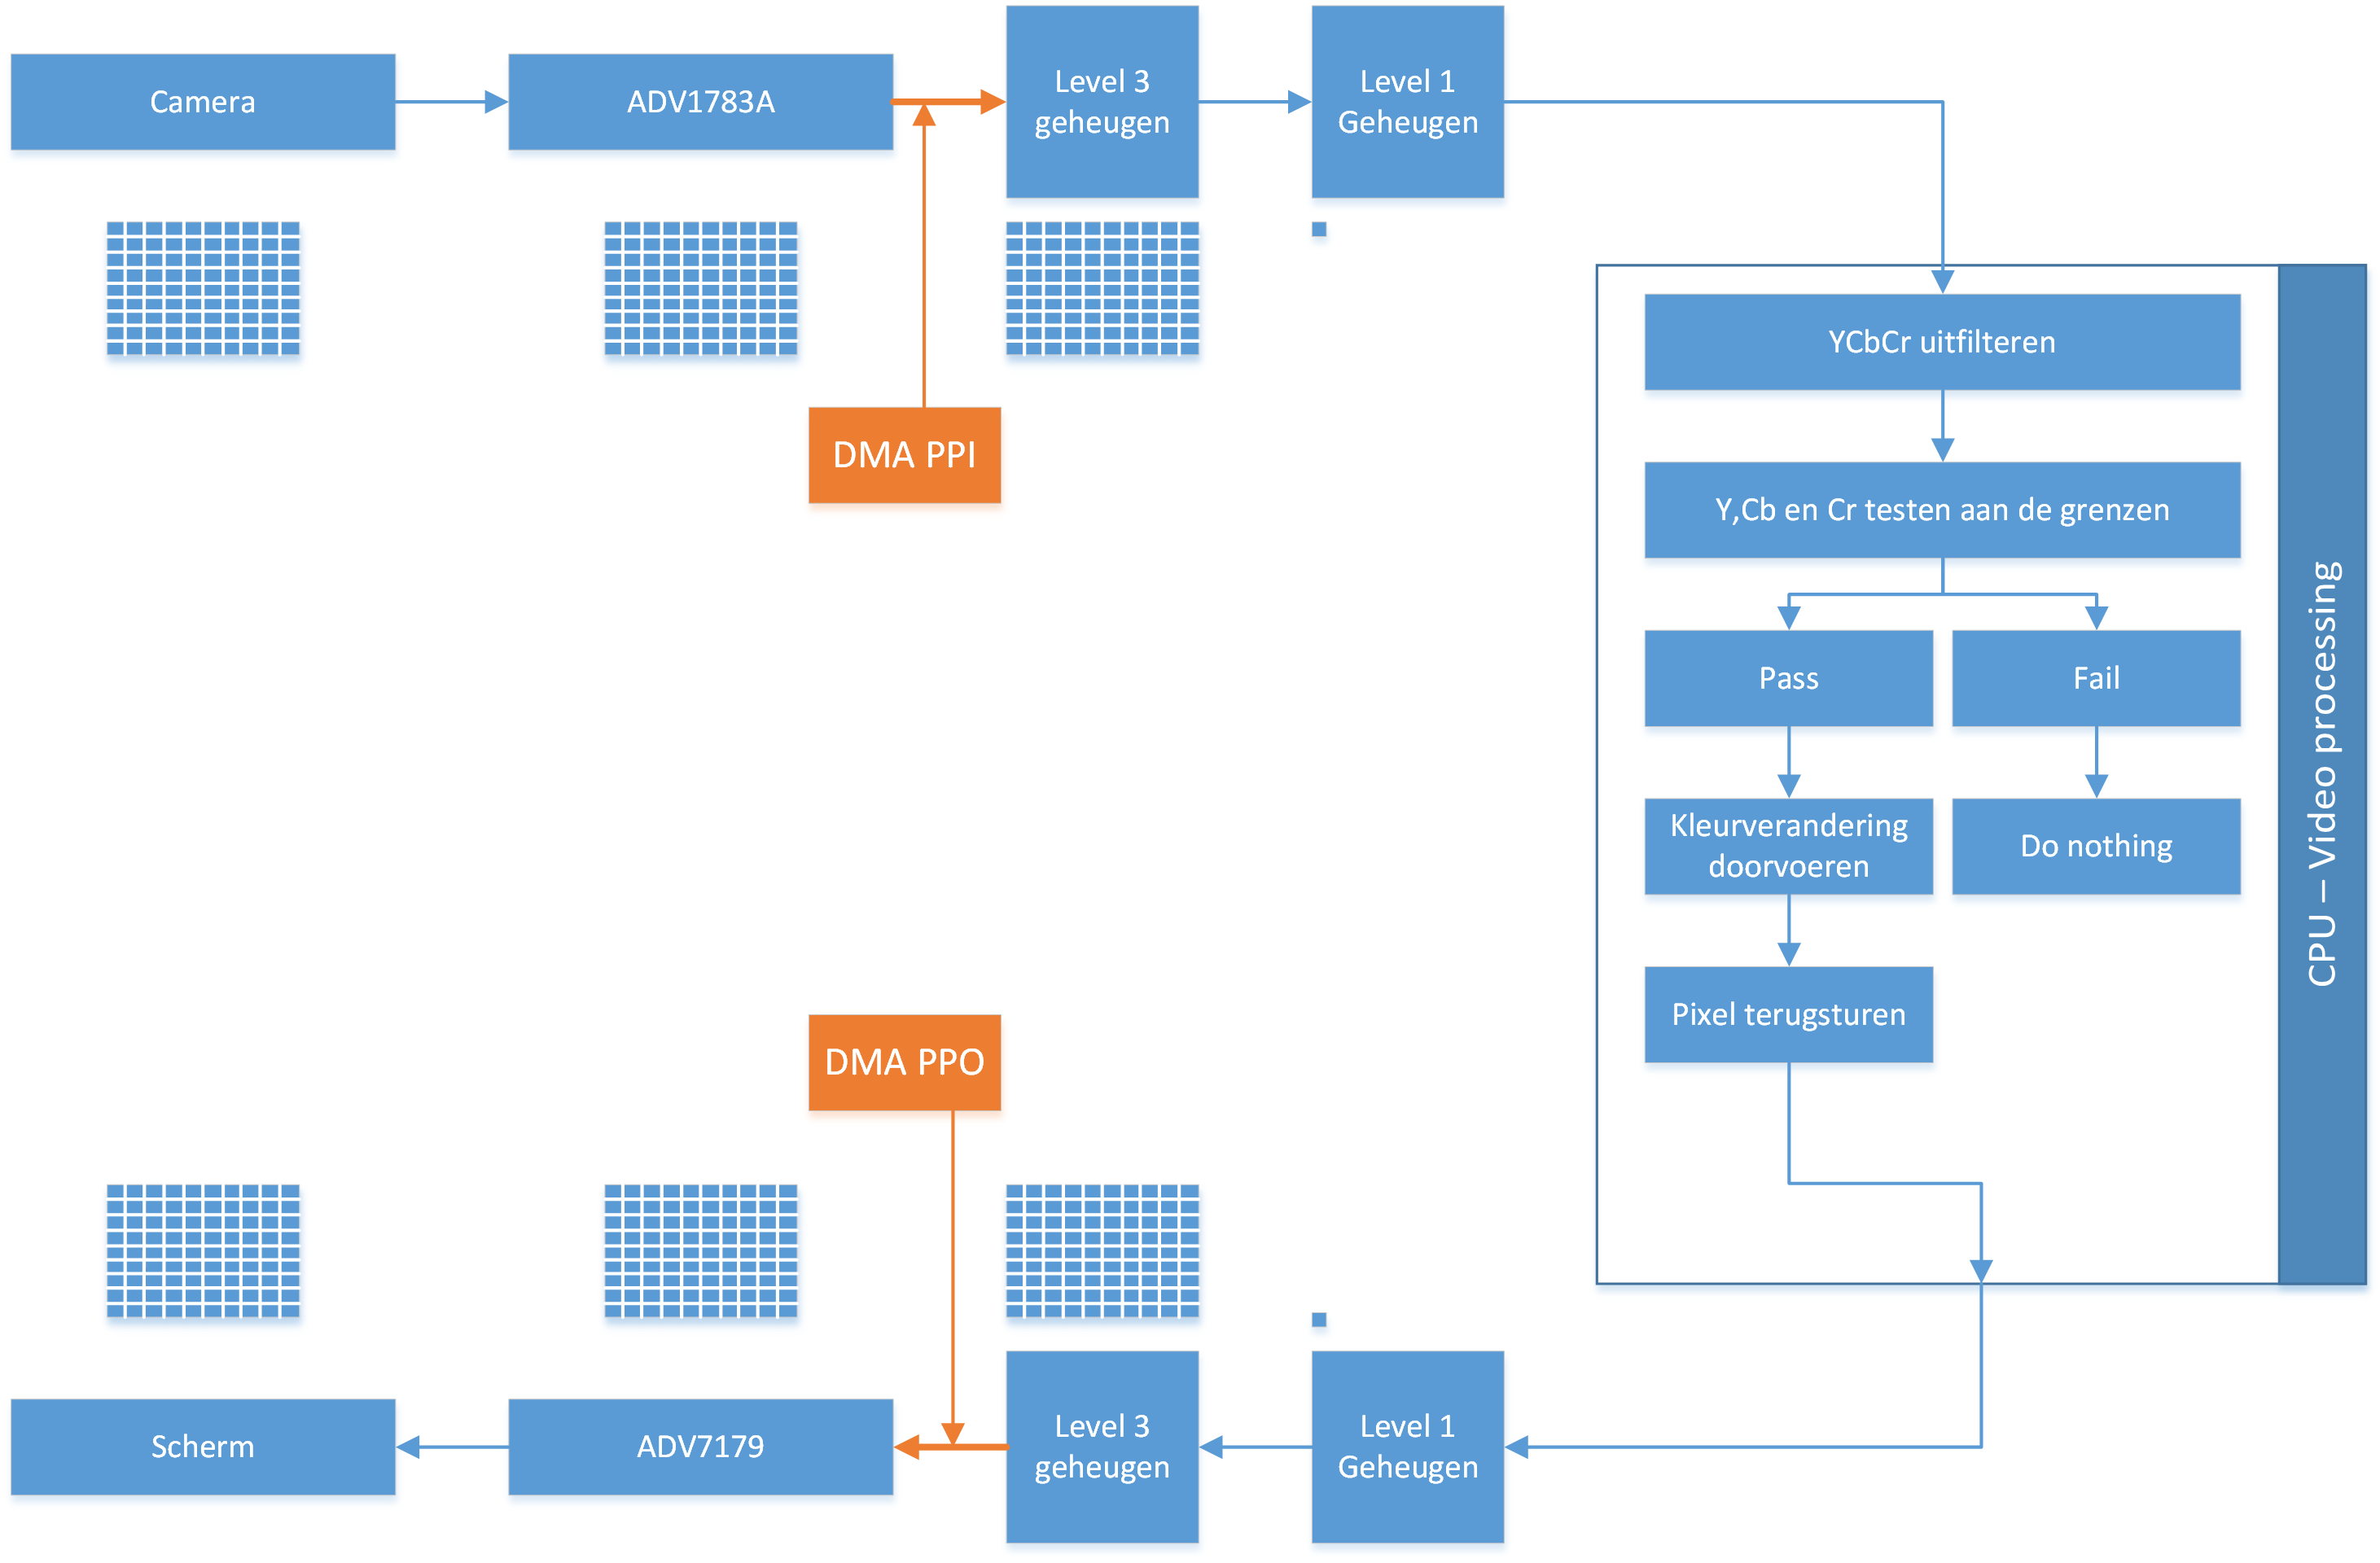
\includegraphics[width=1.0\textwidth]{Chapters/Chapter2/Images/implementationOverview.png}
			\caption{Algemeen overzicht van de implementatie op de BlackFin BF-561}
			\label{fig:algemeenoverzicht}
	\end{figure}
	\newpage
	\par Het algemeen opzet van de implementatie van het algoritme wordt weergegeven in figuur~\ref{fig:algemeenoverzicht}. Deze figuur is eveneens terug te vinden in appendix~\ref{app:algemeenoverzicht}. De videodata wordt binnengelezen van een digitaal fototoestel en via de video decoder die op het EZ-kit aanwezig is wordt deze videodata door middel van PPI opgeslagen in het level 3 SDRAM geheugen. Vervolgens zal door de processor telekens 1 pixel opgevraagd worden om verwerkt te worden. Deze pixel wordt dan gekopieerd naar het level 1 geheugen. Hierna wordt het verwerkingsalgoritme toegepast op de pixel. Dit algoritme zal in de hoofdstukken hieronder verder worden besproken. Indien de pixel van waarde veranderd is na toepassing van het algoritme, dan zal deze terug van het level 1 geheugen naar het level 3 geheugen gestuurd worden. Via de PPO wordt het beeld vervolgens van het level 3 geheugen naar de video encoder gezonden die op zijn beurt het videosignaal doorgeeft aan een scherm.

\section{Frame iteratie}
	\subsection{Active Video Frame}
		\par Om de AVFs te kunnen vinden, moeten we tweemaal met een verschillende offset door de array itereren. Aangezien een lijn ook nog bytes bevat waar men beter niets aan veranderd, is de eenvoudigste oplossing te itereren over de lijnen binnen een frame, en dus telkens de lijnindex te vermenigvuldigen met de lijnlengte (dit is hier 1716 bytes). In elke iteratie van deze loop verkrijgen we een nieuwe lijn. Het eerste AVF bevat de oneven lijnen, en dus zijn dit ook de eerste die we zullen bewerken.
		\smallskip
		\begin{lstlisting}[language=C,caption=Code voor het itereren over een frame]
#define AVSTART1 20
#define AVSTART2 281

for(int avField = 0; avField<2; avField++)
{
	int startFor = (avField==0)?AVSTART1:AVSTART2;
	int endFor = startFor+((avField==0)?AVLENGTH1:AVLENGTH2);
	for(int i=startFor; i<endFor; i++)
	{
		//...
	}
}		\end{lstlisting}

	\subsection{Processing van een beeldlijn}
		\par Een lijn bevat eerst 276 bytes data die we niet mogen overschrijven (Cfr.~\ref{subsec:LijnSubSec}). Pas daarna volgen de 1440 bytes data die wij moeten uitlezen en bewerken. We lezen per iteratie 4 bytes uit omdat deze alle 4 nodig zijn om twee volledige pixels te kunnen bepalen en te converteren naar RGB. Dit zorgt er voor dat we per twee over de array lopen:
		\smallskip
		\begin{lstlisting}[language=C,caption=Code voor her itereren over een lijn]
#define LINEOFFSET 276/2		// 4 EAV + 268 HB + 4 SAV
#define LINELENGTH 1716/2		// ITU-R BT656 line is 1716 bytes

for(j=LINEOFFSET; j<LINELENGTH; j+=2)
{
	//...
}		\end{lstlisting}

\section{Kleurenconversie}
	\subsection{YCbCr naar RGB}
		\par Zoals reeds aangegeven in~\ref{subsec:KleurConversieSubSec}, kunnen we YCbCr perfect converteren naar RGB als we beschikken over vier bytes data die respectievelijk Cb, Y1, Cr en Y2 voorstellen. De input komt binnen onder de vorm van twee shorts, waaruit CbY en CrY gehaald moeten worden. Om dit te bereiken zijn er twee operaties vereist, namelijk shiften en masken, en dit voor beide shorts. Aan de hand van de formules op pagina~\pageref{tab:RGBYCbCrFormulesTable} kunnen we de 4 verkregen bytes omrekenen tot RGB waarden, of in C code:
		\smallskip
		\lstinputlisting[language=C++,caption=YUV naar RGB conversie ge\"implementeert op de BF-561]{Chapters/Chapter2/SourceCode/YUVtoRGB.c}

		\par We cre\"eren een functie die de twee short als argumenten verkrijgt, en na een aantal operaties een jagged array teruggeeft met daarin twee RGB pixelwaarden. Zoals zichtbaar is moet er, om de Cb en Cr te bepalen eerst 8 bit geshift worden naar links. Dit is vereist aangezien ze werwerkt zit in de eerste 8 bits van de short. Om geen onverwachte resultaten te bekomen masken we nog eens met 0xFF zodat we zeker zijn dat de eerste bits allemaal op 0 staan en dus het resultaat niet kunnen be\"invloeden. Om Y1 en Y2 te bepalen is enkel de mask nodig die we als de laatste stap op Cb en Cr ook toegepast hebben. Als laatste combineren we de verkregen waarden in een array en geven deze terug naar waar de aanroep plaatsvond.

	\subsection{RGB naar YCbCr}
		\par RGB naar YCbCr is een heel wat complexere operatie dan de omgekeerde. Dit omdat het berekenen van Y, Cb en Cr een groter aantal operaties vergt. We maken opnieuw een functie, maar ditmaal ontvangt ze de jagged array die gegenereerd wordt in de YCbCr naar RGB conversie als argument, en geeft ze een array van 2 shorts terug, die dan de 2 pixels voorstellen in de YCbCr kleurenruimte.
		\smallskip
		\lstinputlisting[language=C++,caption=todo]{Chapters/Chapter2/SourceCode/RGBtoYUV.c}

		De berekening om de RGB waarden om te zetten naar YCbCr is te vinden in de tabel~\ref{tab:RGBYCbCrFormulesTable} op pagina~\pageref{tab:RGBYCbCrFormulesTable}. Deze passen we toe op de RGB waarden in de binnenkomende array. Deze array is van het formaat {{R,G,B},{R,G,B}} en bevat dus telkens twee pixels. Als laatste stap moeten we de Y, Cb en Cr waarden samenvoegen tot twee shorts die respectievelijk CbY en CrY voorstellen. Om Cb toe te kennen aan de hoogste 8 bit van de short, stellen we CbY eraan gelijk en shiften we ditmaal 8 bits naar links, dus te tegenovergestelde operatie als in de YCbCr naar RGB conversie. Daarna tellen we Y erbij op om deze in de laagste 8 bits te plaatsen. Deze handeling doen we tweemaal, om beide pixels geconverteerd te hebben.

\section{Eerste iteratie}
	\par Nu we de conversies apart bekeken hebben, en ook de iteratie over het frame volledig beschreven hebben, zijn we in staat om dit samen te voegen tot \'e\'en werkend geheeld. Deze code is toegevoegd in bijlage~\ref{app:codesnippet1} op pagina~\pageref{app:codesnippet1}. Het probleem dat zich manifesteerde bij het analyseren van deze code was dat de processing tijd per frame te lang was. Hierdoor verkregen we als uitvoer een flikkerend onstabiel beeld. Er werd gezocht naar een oplossing.

\section{Tweede iteratie}
	\par In een tweede iteratie werd als eerste de conversie van RGB naar YCbCr en omgekeerd verwijderd uit het proces. Dit leverde al een aanzienlijke snelheidswinst op, maar in het worst case scenario waarbij getest werd met een volledig blauw beeld werd slechts 1/4 van het scherm van kleur veranderd. Er is dus meer tijd nodig om een frame volledig te verwerken. Twee mogenlijkheden boden zich aan:

		\begin{enumerate}
			\item Het toepassen van interleaving op de lijnen van het frame. Dit houd in dat in een eerste frame enkel de even lijnen verwerkt worden en in een tweede frame enkel de oneven lijnen.
			\item Het vergroten van de framebuffer geeft de processor meer tijd om een frame te verwerken. Het huidige aantal buffers was 4.
			\item Het samennemen van naast elkaar liggende pixels, om zo het oog te bedriegen.
		\end{enumerate}

	\par Er werd gekozen voor de 2\textsuperscript{e} mogelijkheid. De buffer werd eerst vergroot naar 8 frames, maar dit bleek nog steeds niet voldoende. Wanneer een volledig blauw scherm aanlegden als videosignaal was de verkregen verwerkingstijd nog steeds te kort. Hierna werd overgeschakeld naar een buffering van 32 frames. De verwerkingstijd werd nu aanzienlijk vergroot. Als nadeel daalde de framerate met factor 4. De frame processing code aangepast zoals te zien is in bijlage~\ref{lis:video_A.c}.

	\par De derde mogelijkheid, die ervoor zorgt dat door het checken van een enkele pixel er meerdere pixels tegelijk aangepast worden, was perfect mogelijk en hebben we ook toegepast op deze code. Aan het resultaat was duidelijk te zien dat er een versnelling was in de verwerkingstijd, maar ook dat de resolutie van het schemr als het ware gedeeld werd door 4. Het werkt namelijk zo: er wordt ge\"itereerd over het frame zoals reeds gebeurde, ditmaal echter verspringt de teller steeds per 2 pixels per lijn. Op die manier wordt er dus telkens een pixel overgeslagen. Indien een pixel voldoet aan de eisen om van kleur verandert te worden, worden de naast-, onder- en rechtonderliggende pixels ook meteen vervangen. Dit wil dus ook zeggen dat we enkel de oneven lijnen moeten doen. Zo kan de totale iteratietijd gedeeld worden door 4. De uiteindelijke resolutie is echter zo erbarmelijk dat we besloten dit niet in de uiteindelijke code te behouden.Aangezien we de code geschreven hebben, en ze ook effectief werkt, is ze te zien in bijlage~\ref{lis:video_A_block.c}.

	\par In de code in bijlage~\ref{lis:video_A.c} is niet alleen de kleurenconversie verdwenen, maar is ook een optimalisatie uitgevoerd om het aantal for-iteraties te verminderen. Zo worden AV field 1 en AV field 2 in eenzelfde for-iteratie overlopen. Van de 32 buffers die ter beschikking staan worden er slechts 8 overlopen om de processor meer tijd te geven om deze verwerking te voltooien. Hieraan is ook de framerate verlaging met factor 4 te wijten.

	\par Om deze buffering te vergroten, zijn meer aanpassingen nodig dan enkel in de source files. De buffers worden namelijk op vaste adressen geplaatst om en zo ideaal mogelijk systeem te bekomen. Aangezien het aantal buffers sterk gestegen is, moet deze mapping volledig herzien worden, en dit gebeurt in de linker file. Om het overzicht te bewaren zijn enkel de regels die aangepast zijn weergegeven in bijlage~\ref{lis:video_in_out.ldf}. Daar is te zien hoe er 32 banken voorzien worden van elk 2MB groot. De verklaring voor deze grootte is te lezen in hoofdstuk~\ref{sec:dmacontroller}.
	De frames waarin de data opgeslagen wordt bevinden zich in in het level 3 geheugen, dus ook daar moeten aanpassingen gebeuren. Deze aanpassingen bevinden zich in de files L3\textunderscore SDRAM.h, L3\textunderscore SDRAM.c en uiteindelijk ook system.h. De bekomen code is te zien in respectievelijk bijlagen~\ref{lis:L3_SDRAM.h}, ~\ref{lis:L3_SDRAM.c} en ~\ref{lis:system.h}.

	\par Bronnen:~\cite{bib_12},~\cite{bib_13},~\cite{bib_11}
\chapter{Theoretische methodes}

	\par Een probleem dat zich kan voordoen bij de ge\"implementeerde methode is dat ook de kleur van andere blauwe objecten gewijzigd wordt. Wanneer het blauw eenmaal binnen de ingestelde grenzen valt zal het van kleur veranderd worden. Om dit probleem op te lossen kan gebruik gemaakt worden van een techniek die het mogelijk maakt om objecten realtime in video te herkennen. Wanneer er dan een smurf op het beeldfragment herkend wordt zal enkel dit deel van het beeldfragment een koerswijziging ondergaan. Deze techniek brengt ook onmiddellijk een tweede voordeel met zich mee omdat niet elk beeld volledig, pixel per pixel, overlopen dient te worden om na te gaan of de pixel binnen de ingestelde kleurgrenzen past. 

	\par Wanneer men enkel werkt met de intensiteit van een pixel (RGB, YUV, YCbCr\ldots) dan wordt dit naar aantal bewerkingen vaak groot en zwaar voor de processor wanneer men elke pixel \'e\'en voor \'e\'en moet doorlopen. Dit vormt een probleem wanneer er gebruik gemaakt wordt van realtime video. Om het aantal processor instructies te reduceren is dus een andere techniek nodig. Het gebruik van wavelets biedt een oplossing voor bovenstaand probleem, en maakt het tevens ook mogelijk om de objectdetectie uit te voeren.

	\par Een andere weg die gevolgd kan worden is om wel pixel-per-pixel te werken maar de datastroom op een andere manier aan de processor aan te bieden. In de huidige implementatie wordt telkens een beeld opgevraagd uit het level 3 geheugen van de processor. Dit is een zeer dure operatie wat betreft instructies. Door slim om te springen met de DMA-controller kan men de toevoer van data versnellen en zo het aantal instructies aanzienlijk verminderen. 

\section{Objectdetectie aan de hand van Haar-like-features}

	\par Een relatief eenvoudige techniek die gebruikt wordt om objecten te detecteren is de haar-cascade. Deze techniek maakt gebruik van Haar-like-features om objecten te detecteren. Een ge\"isoleerde pixel bevat enkel informatie over de luminantie en kleur van die bepaalde pixel. Het vertelt niets meer over de structuur of het uitzicht van het geheel. Om meer informatie te krijgen over het geheel dient men een aantal aangrenzende pixels te aanschouwen als een verzameling. Het Viola-Jones algoritme is een feature-based algoritme dat in tegenstelling tot een pixel-based algoritme gebruik maakt van features om objecten te detecteren. Het algoritme maakt gebruik van Haar wavelets. Dit type wavelet laat toe om visuele patronen te beschrijven als een luminantieverandering op verschillende frequenties.

	\par Het Viola-Jones algoritme is ook zelflerend en kan getraind worden door middel van een oefenset afbeeldingen die zowel positieve als negatieve afbeeldingen bevat. zo$'$n model wordt een classificator genoemd en bestaat typisch uit enkele honderdtallen positieve en enkele negatieve afbeeldingen.

	\par Om een classificator aan te maken, wat ook wel training van een classificator genoemd wordt, wordt een wavelet transformatie uitgevoerd op de trainingsafbeelding aan de hand van een haar-like-feature. Om dit proces te versnellen wordt niet de originele afbeelding gebruikt, maar de integraalafbeelding. Een integraalafbeelding kan als volgt gegenereerd worden. De waarde van de pixel op positie x,y van de integraalafbeelding is gelijk aan de waarden van alle pixels met kleinere x- en y-waarden op de originele afbeelding. Vervolgens zullen de pixels van de integraalafbeelding getest worden door middel van een venster dat over de integraalafbeelding heenschuift. Elke feature heeft na deze fase een bepaalde wegingsfactor. Een geheel van deze wegingsfactoren omschrijft dan op zijn beurt een bepaald object.

	\par De integraalafbeelding wordt getest met de haar-like features die weergegeven zijn in figuur~\ref{fig:HaarFeatureImage} op pagina ~\pageref{fig:HaarFeatureImage}. Afhankelijk van de vereiste nauwkeurigheid zal al dan niet de hele set overlopen worden. Dit wordt ook wel eens haar-cascade genoemd. Een model bestaat dus uit een aaneenschakeling van verschillende haar-like-features. 

		\begin{figure}[H]
			\centering
			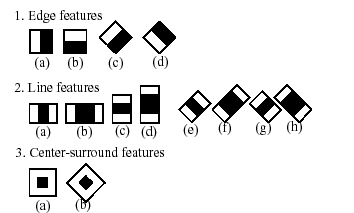
\includegraphics[width=0.65\textwidth]{Chapters/Chapter3/Images/haarfeatures.png}
			\caption{Set van haar-like features die gebruikt worden voor objectdetectie (Bron: http://docs.opencv.org)}
			\label{fig:HaarFeatureImage}
		\end{figure}

	\par Het Viola-Jones algoritme maakt gebruik van bovenstaand model dat opgebouwd is uit haar-like-features om te evalueren of een inkomend beeld het te detecteren object bevat. Alvorens de wavelet op een beeldfragment wordt toegepast, zal eerst een luminantie normalisatie doorgevoerd worden. Hierna zal het beeld verkleind worden tot een resolutie om het verwerkingsproces te versnellen. Vervolgens zal de wavlettransformatie van de afbeelding, die analoog verloopt met het trainen van een model, doorlopen worden en vergeleken worden met het model om zo te evalueren of het te detecteren object op de afbeelding staat. Vervolgens kan ook de positie en grootte (onder de vorm van een rechthoekig gebied) weergegeven worden. 

	\par Wanneer er dus een smurf op de afbeelding gedetecteerd word dan pas dient er op het gedeelte van waar de smurf gedetecteerd is een kleurverandering toegepast te worden. Die detectie van smurfen kan uitgevoerd worden door Core A en de effectieve kleursverandering kan uitgevoerd worden door Core B.

	\par Bovenstaand algoritme is relatief eenvoudig te implementeren op de BlackFin processor omdat de BlackFin Image Processing Toolbox een reeks tools bevat die speciefiek ontworpen zijn om Haar-features toe te passen. Deze toolbox is qua werking en opzet te vergelijken met de OpenCV bibliotheek. 

\section{Slim omspringen met de DMA-controller}
\label{sec:dmacontroller}
	\par Bij de huidige implementatie van de kleurverandering wordt een inkomend beeld telkens opgehaald vanuit het level 3 geheugen. E\'en beeld heeft ongeveer een grootte van 1 \'a 2 MB. Met een beschikbaar geheugen van 64 MB SDRAM kunnen er dus maximum 32 frames gebufferd worden in het SDRAM. De BlackFin beschikt zelf over 32 kB level 1 cache geheugen en 128 kB level 2 cache geheugen. Het voordeel aan dit level 1 en 2 geheugen is dat zij veel sneller aanspreekbaar zijn door de processor dan het relatief trage level 3 geheugen. 

	\par Er valt op te merken dat een volledig frame niet past in het level 1 of 2 geheugen van de BlackFin. Het zou wel mogelijk zijn om een deel van een frame te verplaatsen naar het level 1 of 2 geheugen, dit te verwerken en vervolgens het resultaat weer verplaatsen naar het level 3 geheugen. Deze acties kunnen volbracht worden door de DMA-controller waardoor er geen processorkracht nodig is om deze verplaatsing teweeg te brengen. Dit principe heeft een groot voordeel qua tijd omdat de processor zich enkel moet bezighouden met het bewerken van data, en niet het opvragen ervan. 

	\par Wanneer men de frame-informatie door middel van de DMA lijn per lijn naar het level 2 geheugen kan verplaatsen heeft te processor minder tijd nodig om een lijn te verwerken. Wanneer een lijn eenmaal verwerkt is wordt deze terug naar het level 3 geheugen gestuurd door middel van de DMA-controller. Op deze manier kan mits een aanpassing van de DMA-controller toch de huidige werkwijze van kleurverandering behouden blijven en er toch een grote snelheidswinst geboekt worden. Dit zal een aanzienlijke verbetering van de framerate teweegbrengen.

\chapter{Besluit}
\par We zijn vertrokken uit de template die gebruik maakt van de interframe techniek. Omdat de verwerking ons nog niet helemaal duidelijk was, zijn we daar ook bij gebleven. Het eerste wat we geprobeerd hebben is een ingangssignaal van de camera te tonen op een scherm via het BlackFin bord. Ook DMAs waren nog niet aan ons besteed. Deze zouden pas later hun nut en nood bewijzen. Hier was het grootste struikelblok het frame zelf. Want er zijn tegenstrijdige standaarden voor verschillende toestellen te vinden. Verder zijn er ook delen van de frame data die niet mogen overschreven worden. De meeste tijd in deze fase sloop in het begrijpen van de frame-indeling.

\par Eens we een stabiel beeld verkregen op het scherm was het tijd om een kleur te vervangen door een andere. Iedereen begrijpt dat dit inhoudt dat je kijkt naar elke pixel in het beeld en beslist of deze pixel binnen de grenzen valt van de gekozen kleur, zo ja vervang je ze, zo nee doe je er niks mee. Zoals voorzien werd code geschreven voor de kleurconversie. Toen nog in RGB. En vanaf dat we begonnen met de kleurconversie werd het beeld opnieuw onstabiel. Meer nog, het was afhankelijk van de hoeveelheid blauw die we wilden vervangen. Dus zomaar pixel na pixel verwerken was te traag.

\par Na wat goede raad van een oud docent, Jurgen Baert, zijn we opnieuw aan de slag gegaan, maar via een compleet nieuwe invalshoek. Namelijk, verlies geen tijd in overbodige berekeningen. We deden de kleurdetectie en -conversie zelf in RGB, terwijl het video signaal zelf YCbCr is. Dus verloren we twee keer tijd. En erg veel tijd zelfs, want de conversies tussen kleurenruimtes zijn floating point bewerkingen op een fixed point processor. Erg duur in tijd.

\par Een tweede idee was om meervoudige buffering toe te passen. Daarvoor zijn we dan ook eens erg minutieus de template gaan bestuderen. Initieel waren er 4 frames voorzien om te bufferen. En we hadden op verschillende plaatsen gelezen dat veel bufferen een goed idee was. Daarom werd het aantal buffers met de nodige hindernissen opgetrokken naar 32. Maar helaas niet meteen met een goed resultaat.

\par De betere resultaten kwamen er pas nadat we de schikking van de buffers ook zo wisten te regelen dat er nooit meer een onaangepast frame naar buiten gestuurd werd. Elk frame dat naar buiten ging werd dus verwerkt. Dit had wel een dramatische daling in framerate tot gevolg. Later werd dit echter wat weggewerkt door een betere schikking van de frameselectie voor verwerking. Er werd ook nog geoptimaliseerd op de kleurverwerking, dit was mogelijk omdat Cb geen bovengrens nodig bleek te hebben, aangezien deze grens gewoon de maximale waarde was. Op empirische wijze zijn we dan tot de meest geschikte grenzen gekomen.

\par Verder is er ook een vrij steile leercurve om goed met de BlackFin borden om te leren gaan. Documentatie is moelijk tot onmogelijk te vinden. Maar hoe beter we begrijpen hoe het werkt hoe beter de resultaten zijn. We stellen dus vast dat het echt wel mogelijk is om met de BlackFin borden aan video verwerking en bewerking te doen, zoals te zien is in de code en het resultaat van onze opdracht.



% Indien er bijlagen zijn:
\appendixpage*
\appendix
\addtocontents{toc}{\protect\newpage}
\chapter{Appendix 1}
\section{Codesnippet 1}
	\lstinputlisting[language=C++,caption=Totaalverzicht van de YUV-RGB conversie en frame-iteratie, label = app:codesnippet1]{Chapters/Chapter2/SourceCode/RGBtoYUVcomplete.c}

\newpage
\section{Codesnippet 2}
\lstinputlisting[language=C++,caption=Kleurenconversie met enkele iteratie, label=lis:video_A.c]{Chapters/Chapter2/SourceCode/video_A.c}

\newpage
\section{Codesnippet 3}
\lstinputlisting[language=C++,caption=Aanpassingen aan de linker file voor 32-dubbele buffering, label=lis:video_in_out.ldf, firstline=374, lastline=405]{Chapters/Chapter2/SourceCode/video_in_out.ldf}

\newpage
\section{Codesnippet 4}
\lstinputlisting[language=C++,caption=Aanpassingen aan system.h voor 32-dubbele buffering, label=lis:system.h]{Chapters/Chapter2/SourceCode/system.h}

\newpage
\section{Codesnippet 5}
\lstinputlisting[language=C++,caption=Aanpassingen aan L3\textunderscore SDRAM.h voor 32-dubbele buffering, label=lis:L3_SDRAM.h]{Chapters/Chapter2/SourceCode/L3_SDRAM.h}

\newpage
\section{Codesnippet 6}
\lstinputlisting[language=C++,caption=Aanpassingen aan L3\textunderscore SDRAM.c voor 32-dubbele buffering, label=lis:L3_SDRAM.c]{Chapters/Chapter2/SourceCode/L3_SDRAM.c}

\newpage
\section{Codesnippet 7}
\lstinputlisting[language=C++,caption=Kleurenconversie met pixel skipping, label=lis:video_A_block.c]{Chapters/Chapter2/SourceCode/video_A_block.c}

\chapter{Appendix 2}
\newpage
\section{Algemeen overzicht}
\label{app:algemeenoverzicht}
	\begin{figure}[H]
		\centering
		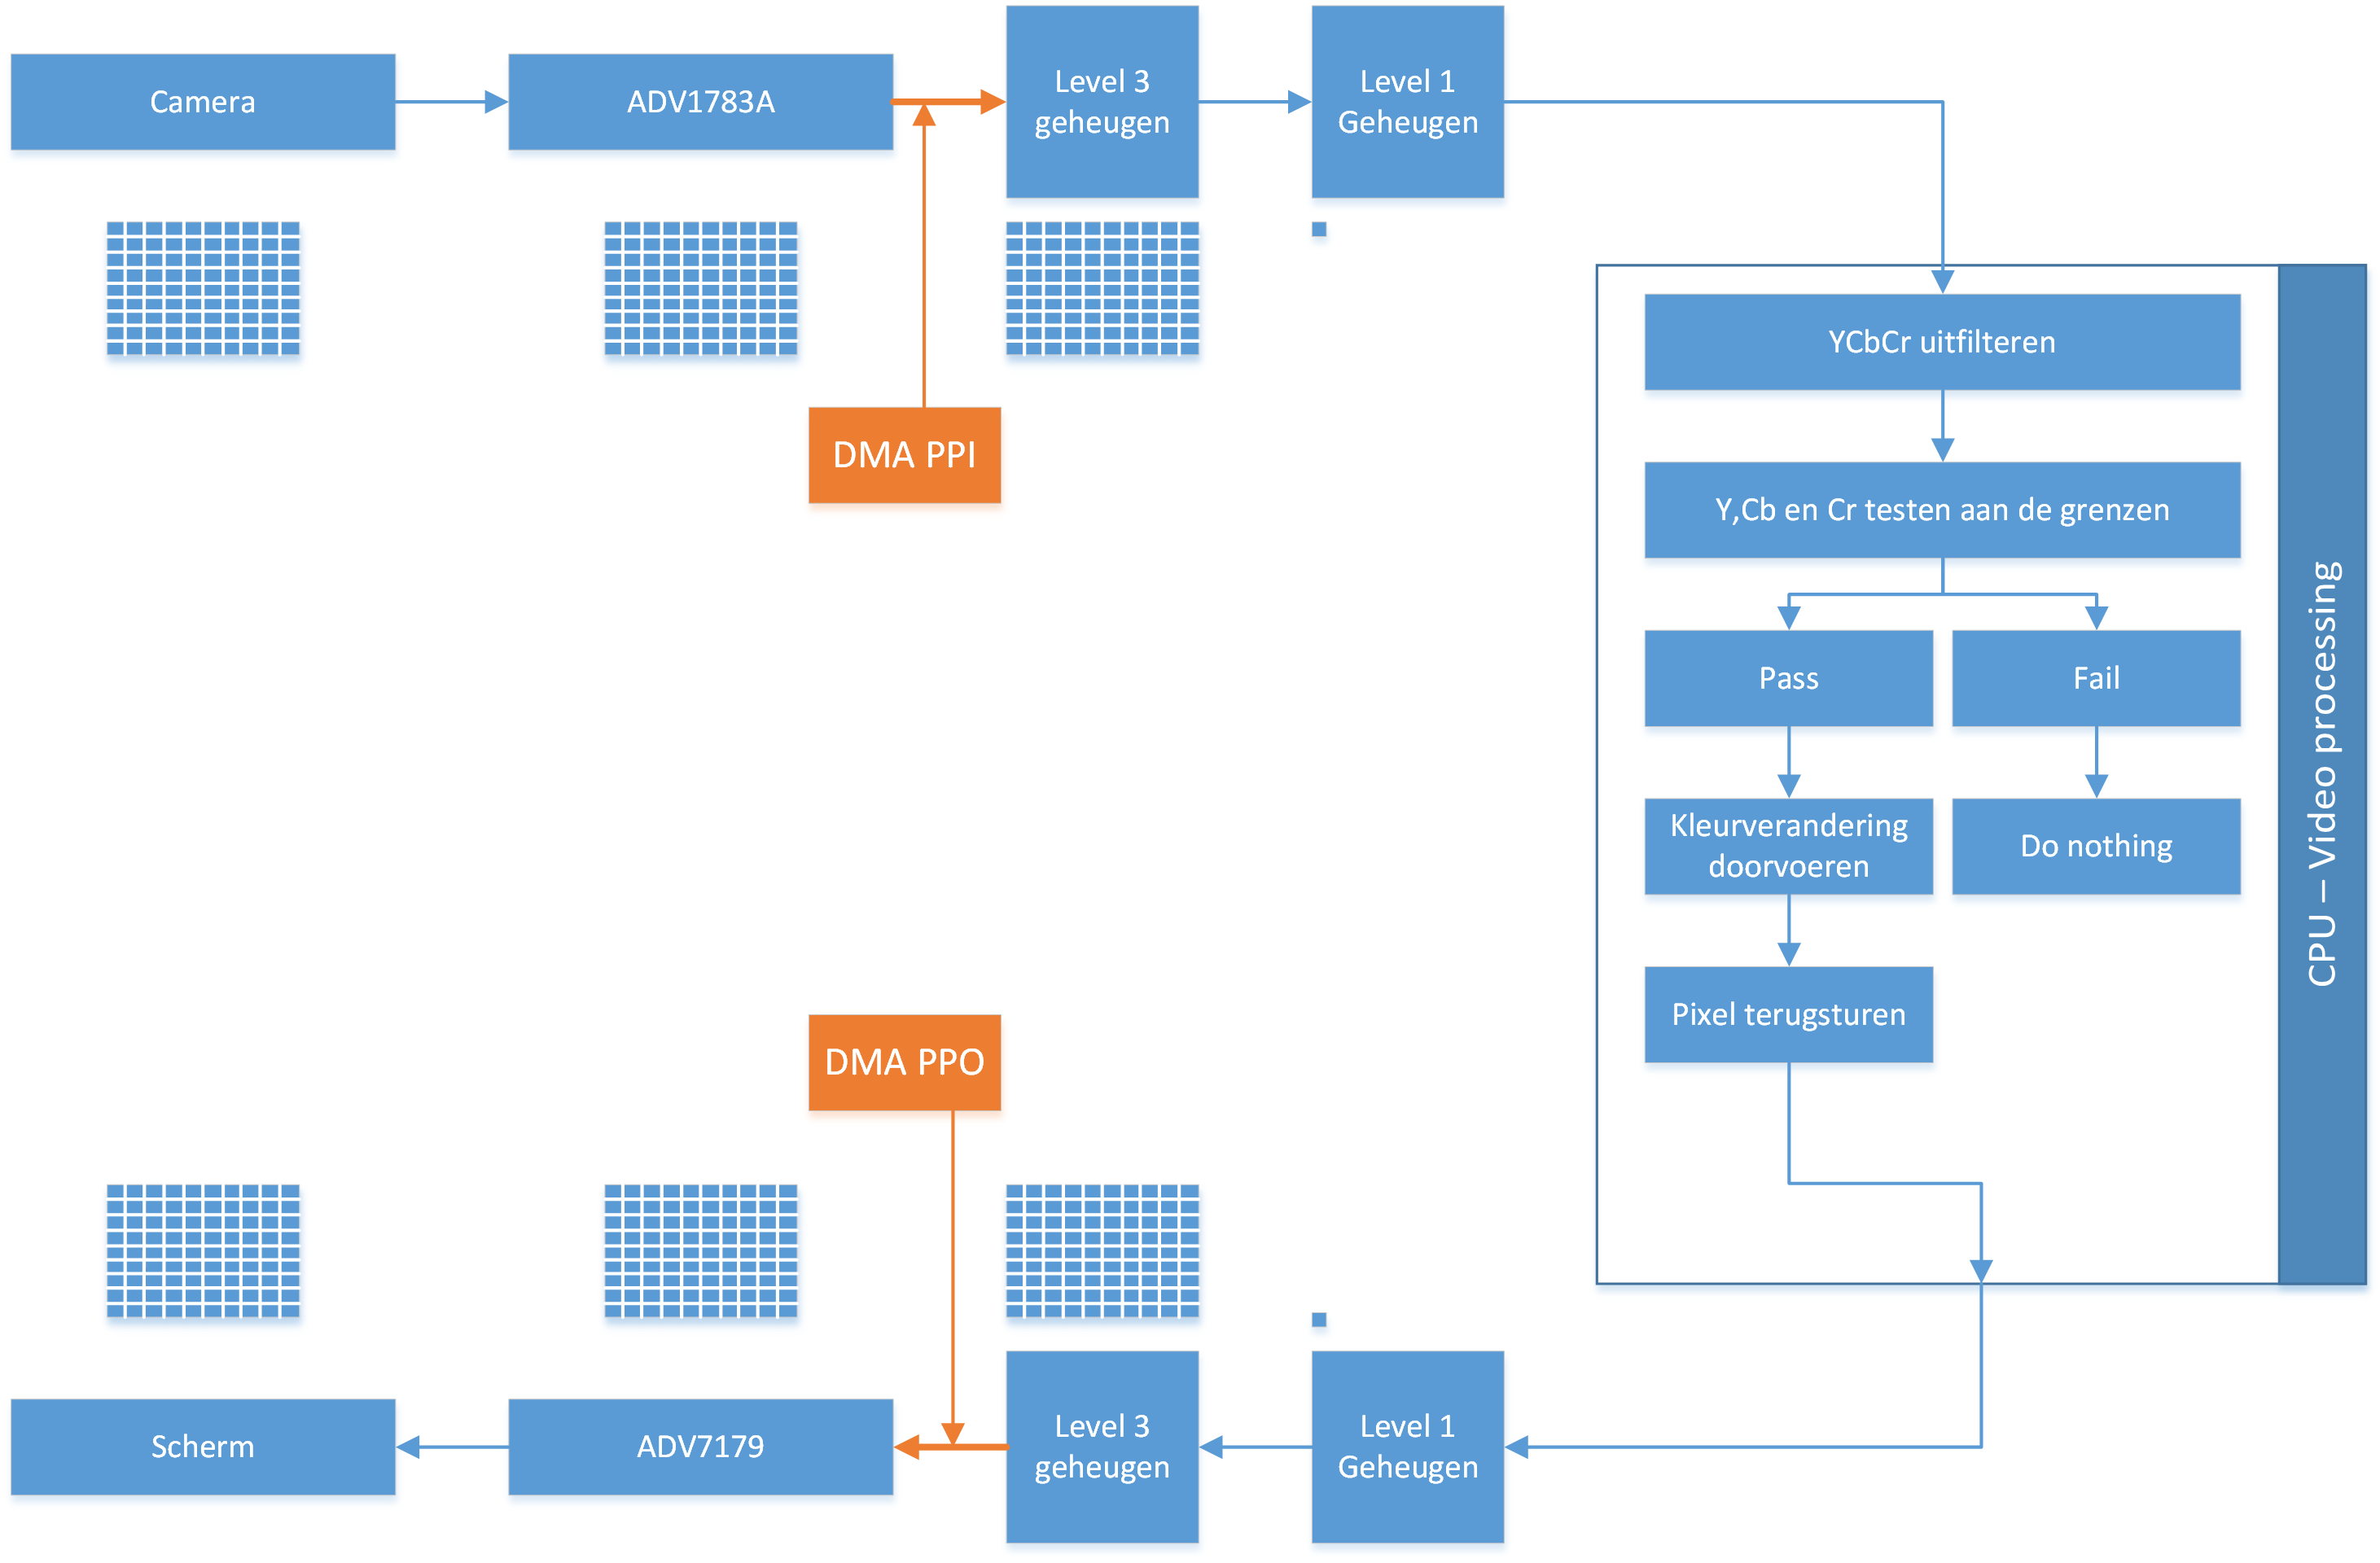
\includegraphics[width=19cm, angle = 90]{Chapters/Chapter2/Images/implementationOverview.png}
		\caption{Algemeen overzicht van de implementatie op de BlackFin BF-561}
	\end{figure}



\backmatter

\bibliographystyle{abbrv}
\bibliography{Sources/references}

\end{document}